\documentclass[reprint,english,notitlepage,aps,nobalancelastpage,nofootinbib]{revtex4-1}  % defines the basic parameters of the document
% if you want a single-column, remove reprint

% allows special characters (including æøå)
\usepackage[utf8]{inputenc}
%\usepackage [norsk]{babel} %if you write norwegian
\usepackage[english]{babel}  %if you write english
\usepackage[T1]{fontenc}


%% note that you may need to download some of these packages manually, it depends on your setup.
%% I recommend downloading TeXMaker, because it includes a large library of the most common packages.

\usepackage{physics,amssymb}  % mathematical symbols (physics imports amsmath)
\usepackage{graphicx, bm}         % include graphics such as plots
\usepackage{upgreek}
\usepackage{float}
\usepackage{xcolor}           % set colors
\usepackage[hidelinks]{hyperref}         % automagic cross-referencing (this is GODLIKE)
\usepackage{tikz}             % draw figures manually
\usepackage{listings}         % display code
\usepackage{subfigure}        % imports a lot of cool and useful figure commands
\usepackage{verbatim}
\usepackage{adjustbox}
\usepackage{mathpazo}
\usepackage{siunitx}
\usepackage{kantlipsum}
\usepackage{bigints}
\usepackage{multirow}
\usepackage{geometry}
\usepackage{algorithm2e}
\usepackage{amsmath}

% defines the color of hyperref objects
% Blending two colors:  blue!80!black  =  80% blue and 20% black
\hypersetup{ % this is just my personal choice, feel free to change things
    colorlinks,
    linkcolor={red!50!black},
    citecolor={blue!50!black},
    urlcolor={blue!80!black}}

%% Defines the style of the programming listing
%% This is actually my personal template, go ahead and change stuff if you want
\lstset{ %
	inputpath=,
	backgroundcolor=\color{white!88!black},
	basicstyle={\ttfamily\scriptsize},
	commentstyle=\color{magenta},
	language=Python,
	morekeywords={True,False},
	tabsize=4,
	stringstyle=\color{green!55!black},
	frame=single,
	keywordstyle=\color{blue},
	showstringspaces=false,
	columns=fullflexible,
	keepspaces=true}

\newcommand\numberthis{\addtocounter{equation}{1}\tag{\theequation}}
\newcommand{\ihat}{\boldsymbol{\hat{\textbf{\i}}}}
\newcommand{\jhat}{\boldsymbol{\hat{\textbf{\j}}}}
\newcommand{\khat}{\boldsymbol{\hat{\textbf{k}}}}
\newcommand{\del}[1]{\textbf{#1)}}
\newcommand{\svar}[1]{\underline{\underline{{#1}}}}
\newcommand{\vc}[1]{\mathbf{#1}}
\renewcommand{\deg}{^{\circ}}
\newcommand{\hksqrt}[2][]{\ \mathpalette\DHLhksqrt{[#1]{#2\,}}}
\def\DHLhksqrt#1#2{\setbox0=\hbox{$#1\sqrt#2$}\dimen0=\ht0
	\advance\dimen0-0.3\ht0
	\setbox2=\hbox{\vrule height\ht0 depth -\dimen0}
	{\box0\lower0.65pt\box2}}

\newcommand{\expy}{\mathbb{E}[\mathbf{\tilde{y}}]}
\newcommand{\expz}{\mathbb{E}[\mathbf{\tilde{z}}]}
\newcommand{\closed}[1]{\left({#1}\right)}
\newcommand{\bracket}[1]{\left[{#1}\right]}


\graphicspath{{../output/plots/}} % search for figures in this dir



\begin{document}


\begin{titlepage}
	\begin{center}
	\textbf{Analysis of Regression and Resampling Methods}

	\vspace{0.2cm}
	Håkon Olav Torvik, Vetle Vikenes and Sigurd Sørlie Rustad

	\vspace{0.5cm}
	
\includegraphics[scale=0.5]{../../pictures/UIO}
	\vspace{0.8cm}

	University of Oslo\\
	Norway\\
	\today	\\
	\end{center}
	\tableofcontents
	\clearpage
\end{titlepage}
%\maketitle                              % creates the title

\onecolumngrid
\section*{Introduction}

Regression analysis is a statistical method for fitting a function to data. It is useful for building mathematical models to explain noisy observations. There are several regression methods to achieve this, all with their strengths and weaknesses. We will in this paper study three different methods; ordinary least squares, Ridge and Lasso regression. All the code, results and instructions on running the code can be found in our GitHub repository\footnote{\href{https://github.com/sigurdru/FYS-STK4155/tree/main/project1}{https://github.com/sigurdru/FYS-STK4155/tree/main/project1}}.

The mathematical model obtained from regression analysis can be used to predict an outcome, given some previously untested input. To build an accurate model, one has to train it on a lot of data. Real-world datasets usually have a fixed size, and getting more data can be practically impossible. Training the model on the same data over and over will usually lead to overfitting, where the model exactly predicts the training set, but performs very poorly on new data. It is therefore useful to have tools to avoid this for small datasets. Resampling methods are such tools. In addition to the regression methods, we will also study the effect of bootstrapping and cross-validating the data.

In order to study this, we need data to analyze. We will in this paper test the methods on two datasets. One dataset we will generate ourselves using a noisy analytical bivariate function, the Franke function \eqref{eq:FF}, while other is real-world terrain data. To both we will be performing a polynomial fit in $x$ and $y$ dependance of the form $[1, x, y, x^2, xy, y^2, \dots]$.

\begin{align}
	\begin{split}\label{eq:FF}
		f(x,y) = &\frac{3}{4}\exp(-\frac{(9x -2)^2}{4} - \frac{(9y-2)^2}{4}) + \frac{3}{4}\exp(-\frac{(9x + 1)^2}{49} - \frac{(9y + 1)}{10})
		\\
		+ &\frac{1}{2}\exp(-\frac{(9x-7)^2}{4} - \frac{(9y -3)}{4}) - \frac{1}{5}\exp(-(9x-4)^2 - (9y-7)^2)
	\end{split}
\end{align}

We will begin with using the simplest regression method, ordinary least squares (OLS) to fit polynomials up to fifth order on the Franke function. At first we will not resample the data, only test our implementation and do some basic analysis. We will then add the resampling methods, Bootstrapping and Cross-Validation. Then we will do the same analyses as before, but using the more complex regression methods Ridge and Lasso. At the end we will do all the same using the terrain data. This paper will not study the effects of different scaling methods, train-test split ratios and amount of noise.

We have also written code to test our implementation of the methods, where we compare our results with those obtained using the open-source machine learning package Scikit-learn. The results from this are presented in Appendix \ref{Apx:test}.

%Tenke me heller plassere dette i Exersice 6 hvor det skal brukes, og ikke i introduksjonen. here\footnote{\href{https://github.com/CompPhysics/MachineLearning/tree/master/doc/Projects/2021/Project1/DataFiles}{https://github.com/CompPhysics/MachineLearning/tree/master/doc/Projects/2021/Project1/DataFiles}}.


\section*{Exercise 1: Ordinary Least Square (OLS) on the Franke function}

We generate a dataset drawing $n=30$ uniformly distributed points in $x, y \in[0, 1]$. Equation \eqref{eq:FF} is then used to create $n^2$ \(z\)-values. In this domain, \eqref{eq:FF} takes values \(z\in[-0.45, \hspace{1mm} 1.52]\) before scaling. To this we add normally distributed stochastic noise. The noise has a mean of $\mu=0$, and variance $\sigma^2=1$. It is scaled by a factor $\epsilon$, which we normally set to $\epsilon=0.2$. This gives a substantial amount of noise, without completely drowning out the data. The data with and without noise is visualized in figure \ref{fig:FF_dataset}.

\begin{figure}[!htb]
	\minipage{0.49\textwidth}
	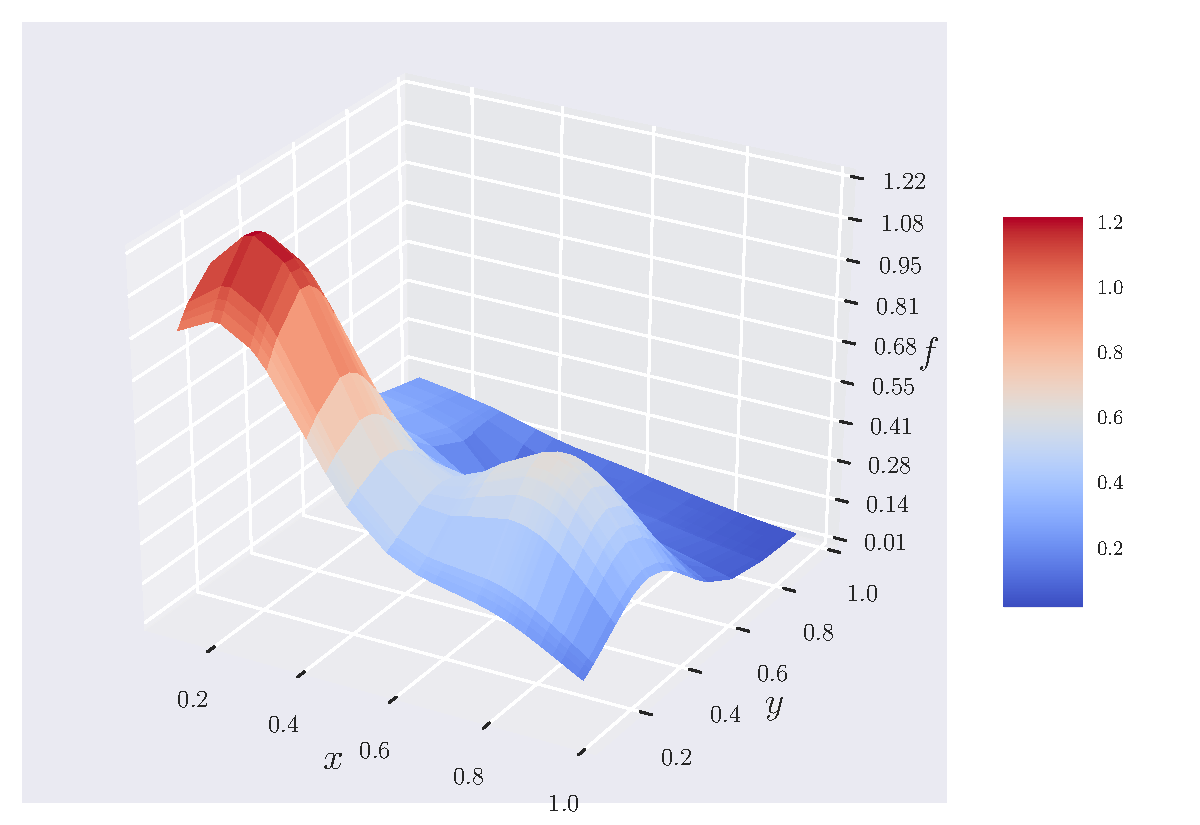
\includegraphics[width=\linewidth]{Frank_anal_eps_0.pdf}
	\endminipage\hfill
	\minipage{0.49\textwidth}
	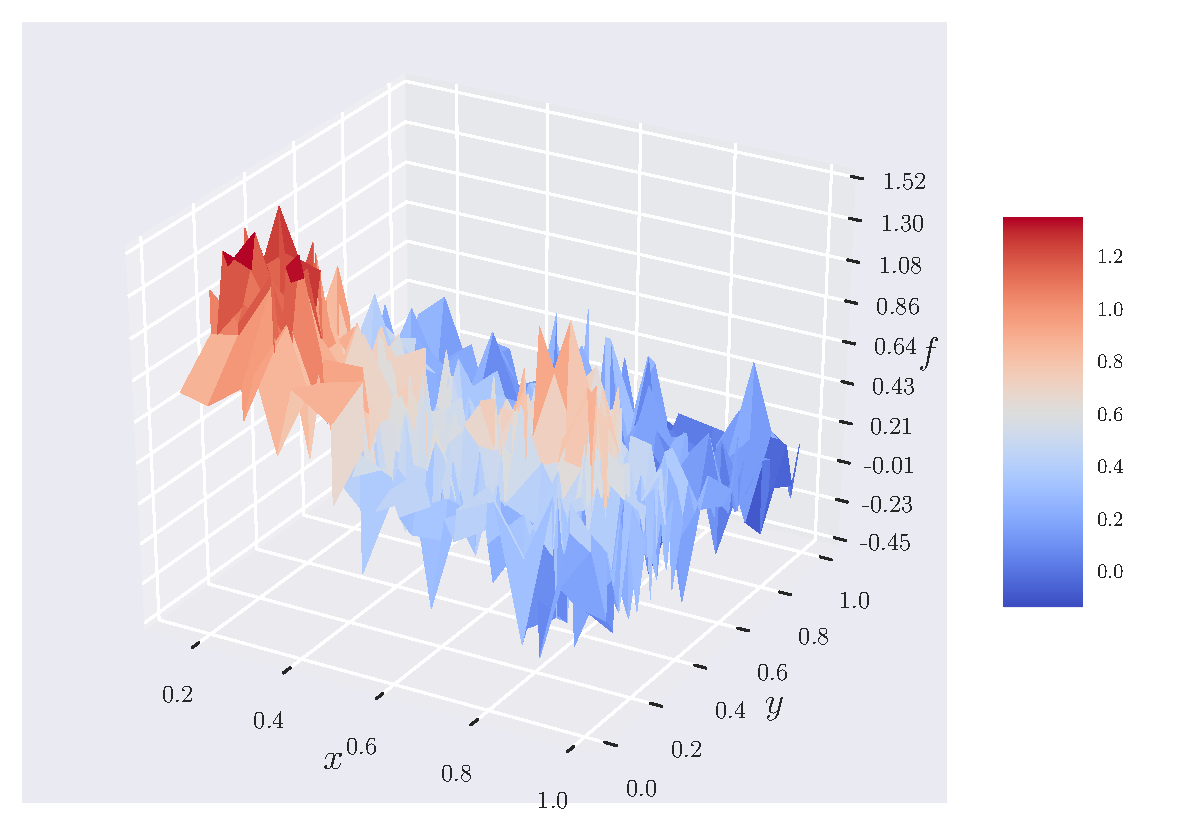
\includegraphics[width=\linewidth]{Franke_rawdata_eps02.pdf}
	\endminipage
	\caption{Here we have displayed our noisy data along with the analytical function. The left figure shows the analytical Franke function, while the right figure is the Franke function with noise.}\label{fig:FF_dataset}
\end{figure}

It is good practice in regression analysis to scale the data, such that different features take values in the same order of magnitude. There are several different methods for scaling, one of which is StandardScaler. This subtracts from the data the mean, and divides by the standard deviation. This centres the data around $0$ and sets the variance to $1$. Because our $x$ and $y$ is already in the domain $[0, 1]$ with variance 1, this only shifts it down, and has no outcome on the regression results. For $z$ generated using \eqref{eq:FF} the effect is small, but we choose to do this for consistency. Our code allows for the following different scaling methods: no scaling, Normalizer and MinMax, though these will not be used.

We are fitting a bivariate polynomial of degree $P$. With $P$ as the highest polynomial degree, the polynomial will have $p=(P+1)(P+2) / 2$ terms. It can, without noise, be written
\begin{equation}\label{eq:zpolynm}
	z(x, y) = \beta_0 + \beta_1x + \beta_2y + \beta_3x^2 + \beta_4xy + \beta_5y^2 + \dots
\end{equation}
where the $\beta$-parameters are coefficients for each term. The $x$ and $y$'s are collected in a design matrix $X$. The columns of $X$ are the terms, while the rows are all terms for a single datapoint. $X$ thus have size $(n^2\cross p)$. The $\beta$s are collected in a vector $\boldsymbol{\beta}$ of length $p$. This is unknown.

Thus, out model with stochastic noise takes the form
\begin{equation}
	\label{eq:z_true_data}
	\vc{z} = X \boldsymbol{\beta} + \boldsymbol{\epsilon},
\end{equation}

One challenge in our case is that our data is two-dimensional, i.e. $\vc{z}$ has dimensions $(n,n)$. We create a workaround by mapping our two-dimensional data, to a one dimensional $(n^2,1)$ vector. This is an important note, and we will do this throughout the report.

We want to create a model to predict $\vc{z}$ given an input. $\boldsymbol{\tilde\beta}$ are the optimal parameters obtained from regression. Our prediction \(\boldsymbol{\tilde{\vc{z}}}\) is then given by

\begin{equation*}
	\boldsymbol{\tilde{z}} = X\boldsymbol{\tilde{\beta}}.
\end{equation*}

To asses the quality of the model, we need a way to quantify the error. We will use the mean square error (MSE), and $R^2$-score, given by

{\large
\begin{align*}
	MSE(\boldsymbol{z}, \boldsymbol{\tilde{z}}) &= \frac{1}{N}\sum_{i=0}^{N-1} (z_i - \tilde{z}_i)^2 = \frac{1}{N}\left\{(\vc{z} - X\boldsymbol{\tilde{\beta}})^T(\vc{z} - X\boldsymbol{\tilde{\beta}})\right\}.
	\\
	R^2(\boldsymbol{z}, \boldsymbol{\tilde{z}}) &= 1 - \frac{\sum_{i=0}^{n-1}(z_i - \tilde{z}_i)^2}{\sum_{i=0}^{n-1}(z_i - \bar{z})^2}, \hspace{3mm} \bar{z} = \frac{1}{n}\sum_{i=0}^{n-1}z_i
\end{align*}
}%

MSE will always be larger than 0, and an MSE of 0 means our model fits the data perfectly. The $R^2$-score is a number between 0 and 1, with 1 being a perfect fit. In order to find the optimal parameters $\boldsymbol{\tilde{\beta}}$ we need a cost function to minimize. Choosing MSE as the cost-function gives the expresion for OLS-regression.
\begin{equation*}
	C(\boldsymbol{\beta}) = MSE(\boldsymbol{z}, \boldsymbol{\tilde{z}})
\end{equation*}
Minimizing this is done by doing the derivative with respect to all the parameters, and finding the zero.
\begin{equation}\label{eq:Const_OLS}
	\frac{\partial C(\boldsymbol{\beta})}{\partial \boldsymbol{\beta}} \equiv 0 = X^T(\boldsymbol{z} - X\boldsymbol{\tilde{\beta}}).
\end{equation}
We can rewrite this as
\begin{equation}\label{eq:OLS_beta}
	X^T\vc{z} = X^TX\boldsymbol{\tilde{\beta}} \implies \boldsymbol{\tilde{\beta}} = (X^TX)^{-1} X^T \vc{z} \equiv \boldsymbol{\hat{\beta}}
\end{equation}
This is OLS-regression. Thus $\boldsymbol{\hat{\beta}}$ are the optimal parameters that minimizes the cost function.

Now that we have an expression for the optimal parameters, we also want to evaluate how good our results are. We do this by splitting our data into two sets, one set for training (80\%) and one set for testing (20\%). We can then find the optimal parameters ($\boldsymbol{\hat{\beta}}$) using the train data, and then compare our test data to the actual data.

%There are many quantities we can use to evaluate our results, however we have decided to calculate the MSE and $R^2$ score. MSE is given by equation \eqref{eq:MSE} and the $R^2$ score by equation \eqref{eq:R2}.
%\begin{equation}
%	\label{eq:MSE}
%	MSE(\vc{z}, \vc{\tilde{z}}) = \frac{1}{n}\sum_{i=0}^{n-1}(z_i - \tilde{z}_i)^2
%\end{equation}
%$MSE(\vc{z}, \vc{\tilde{z}})$ is the mean square between the datapoints $\vc{z}$ and $\vc{\tilde{z}}$.
%\begin{equation}
%	\label{eq:R2}
%	R^2(\vc{z}, \vc{\tilde{z}}) =
%\end{equation}
%Here $R^2(\vc{z}, \vc{\tilde{z}})$ is the $R^2$ score between the datapoints $\vc{z}$ and $\vc{\tilde{z}}$.

We can now perform OLS on our data and plot the MSE and $R^2$-score as a function of polynomial degree. It is important to note that when we fit using a polynomial of degree $p$, all terms from lower polynomial degrees are included in the fit. We expect the MSE to strictly decrease and $R^2$ to strictly increase for the train data, as our model will become more complex. We expect the same for the test data, however at a certain polynomial degree we might se overfitting. This would make our error increase and $R^2$ score decrease. The results are plotted in figure \ref{fig:OLS_R2_and_MSE}. Overfitting is when the model nearly perfectly fits the training data, while performing very poorly on test data.

\begin{figure}[H]
	\minipage{0.49\textwidth}
	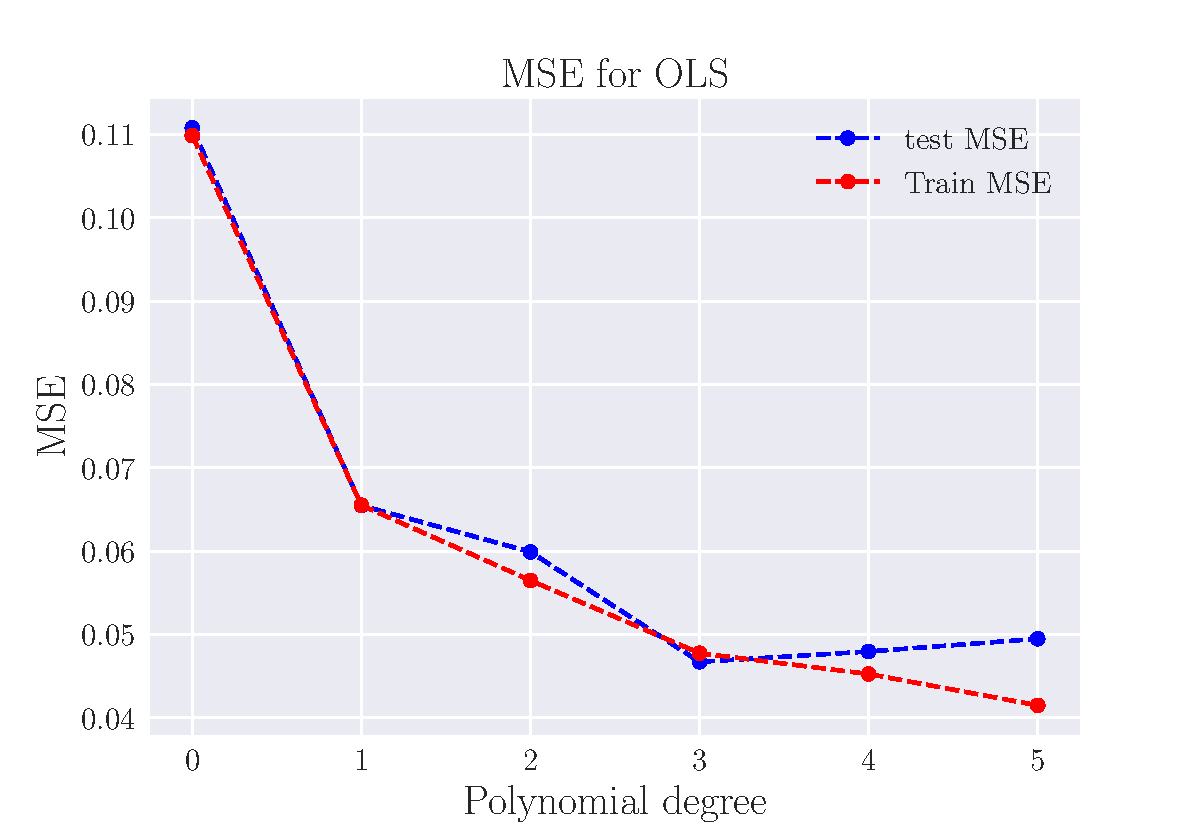
\includegraphics[width=\linewidth]{MSE_OLS_n30_eps02_pol5.pdf}
	\endminipage\hfill
	\minipage{0.49\textwidth}
	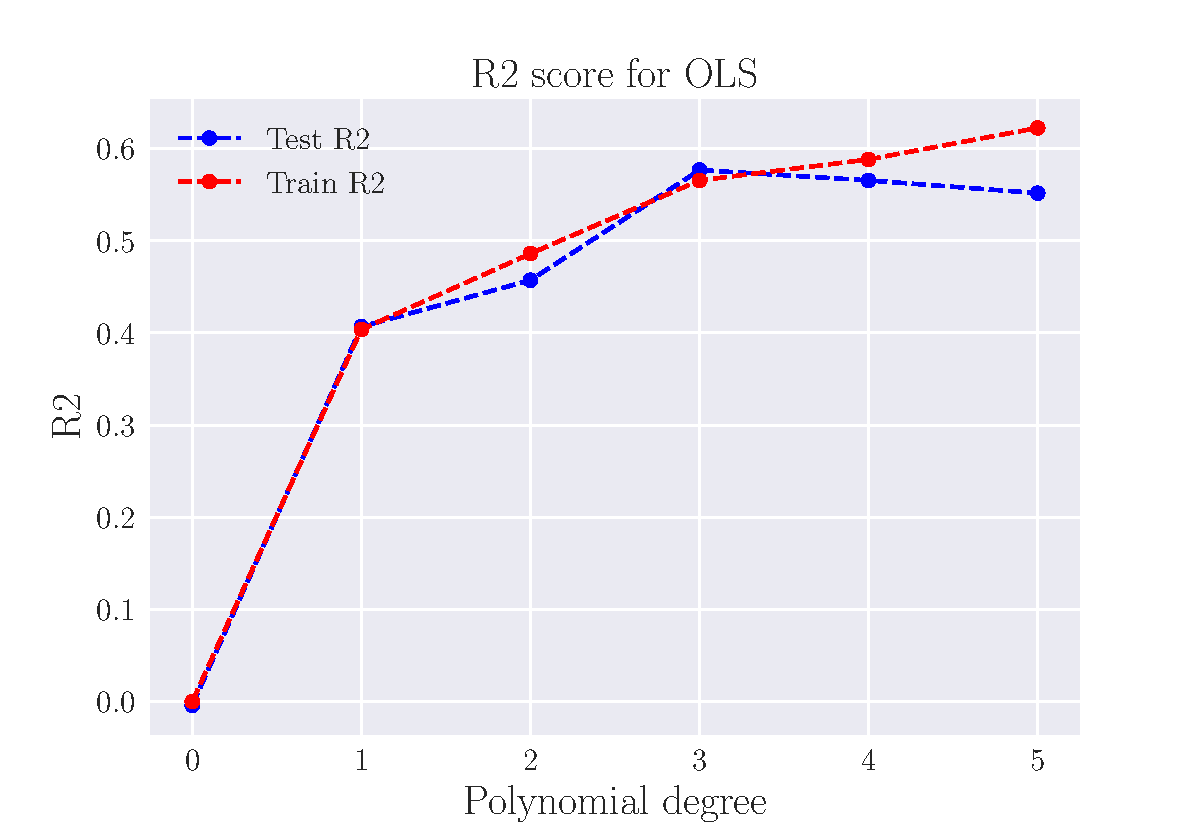
\includegraphics[width=\linewidth]{R2_OLS_n30_eps02_pol5.pdf}
	\endminipage
	\caption{Here we have plotted the MSE and $R^2$-score for OLS. The left figure shows the MSE and right shows the $R^2$ score. The red dotted line is from the train data, and the blue dotted line is from the test data.}\label{fig:OLS_R2_and_MSE}
\end{figure}
From figure \ref{fig:OLS_R2_and_MSE} we see that the MSE strictly decrease and $R^2$-score increase for the test data. This indicates that we have not reached a point of overfitting yet.

It is also interesting to look at the variance in the parameters, because this would give an indication of overfitting. We know that for a set of optimal parameters
$\boldsymbol{\hat{\beta}} = (X^TX)^{-1}X^T \vc{z}$,
We have the expectation value
\begin{equation*}
	\mathbb{E}[\boldsymbol{\hat{\beta}}] = \mathbb{E}[(X^TX)^{-1}X^T \vc{z}] = (X^TX)^{-1}X^T\mathbb{E}[\vc{z}] = (X^TX)^{-1}X^TX\boldsymbol{\hat{\beta}} = \boldsymbol{\hat{\beta}}.
\end{equation*}
With this we can calculate the variance in $\boldsymbol{\hat{\beta}}$.
\begin{align*}
	\text{Var}(\boldsymbol{\hat{\beta}}) &= \mathbb{E}\left[(\boldsymbol{\hat{\beta}} - \mathbb{E}[\boldsymbol{\hat{\beta}}])(\boldsymbol{\hat{\beta}} - \mathbb{E}[\boldsymbol{\hat{\beta}}])^T\right] \\
	&= \mathbb{E}\left[((X^TX)^{-1}X^T\vc{z}- \boldsymbol{\hat{\beta}})((X^TX)^{-1}X^T\vc{z}- \boldsymbol{\hat{\beta}})^T\right] \\
	&= (X^TX)^{-1}X^T \mathbb{E}\left[\vc{z}\vc{z}^T\right]X(X^TX)^{-1}- \boldsymbol{\hat{\beta}}\boldsymbol{\hat{\beta}}^T \\
	&= (X^TX)^{-1}X^T\left[X\boldsymbol{\hat{\beta}}\boldsymbol{\hat{\beta}}^TX^T + \sigma^2 \right] X (X^TX)^{-1} - \boldsymbol{\hat{\beta}}\boldsymbol{\hat{\beta}}^T \\
	&= \boldsymbol{\hat{\beta}}\boldsymbol{\hat{\beta}}^T + \sigma^2(X^TX)^{-1} - \boldsymbol{\hat{\beta}}\boldsymbol{\hat{\beta}}^T = \sigma^2(X^TX)^{-1}
\end{align*}
Here we used $\mathbb{E} (\vc{z}\vc{z}^T) = X \boldsymbol{\hat{\beta}}\boldsymbol{\hat{\beta}}^T X^T + \sigma^2\mathbb{1}$, where $\sigma^2 = \epsilon = 0.2$ is the variance of the noise and $\mathbb{1}$ is the identity. Now we have an estimate for the variance in parameter $\boldsymbol{\hat{\beta}}_{j}$ given by
\begin{equation}
	\boldsymbol{\sigma}^2(\boldsymbol{\hat{\beta}}_{j}) = \sigma^2 [(X^TX)^{-1}]_{jj}.
	\label{eq:var_OLS}
\end{equation}
Using equation \eqref{eq:var_OLS} we can plot the confidence interval for the different parameters, for several polynomial degrees (see figure \ref{fig:var_beta}).
\begin{figure}[H]
	\minipage{0.49\textwidth}
	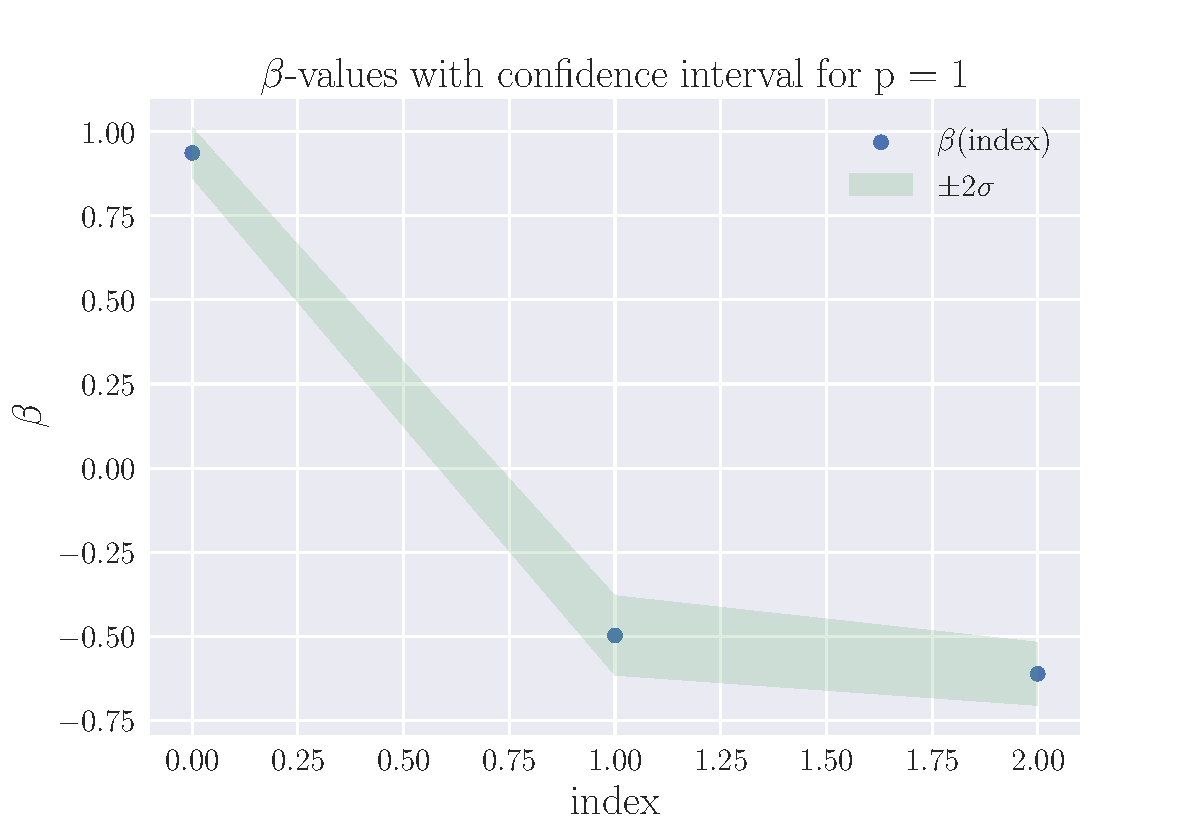
\includegraphics[width=\linewidth]{Var_OLS_poldeg_1.pdf}
	\endminipage\hfill
	\minipage{0.49\textwidth}
	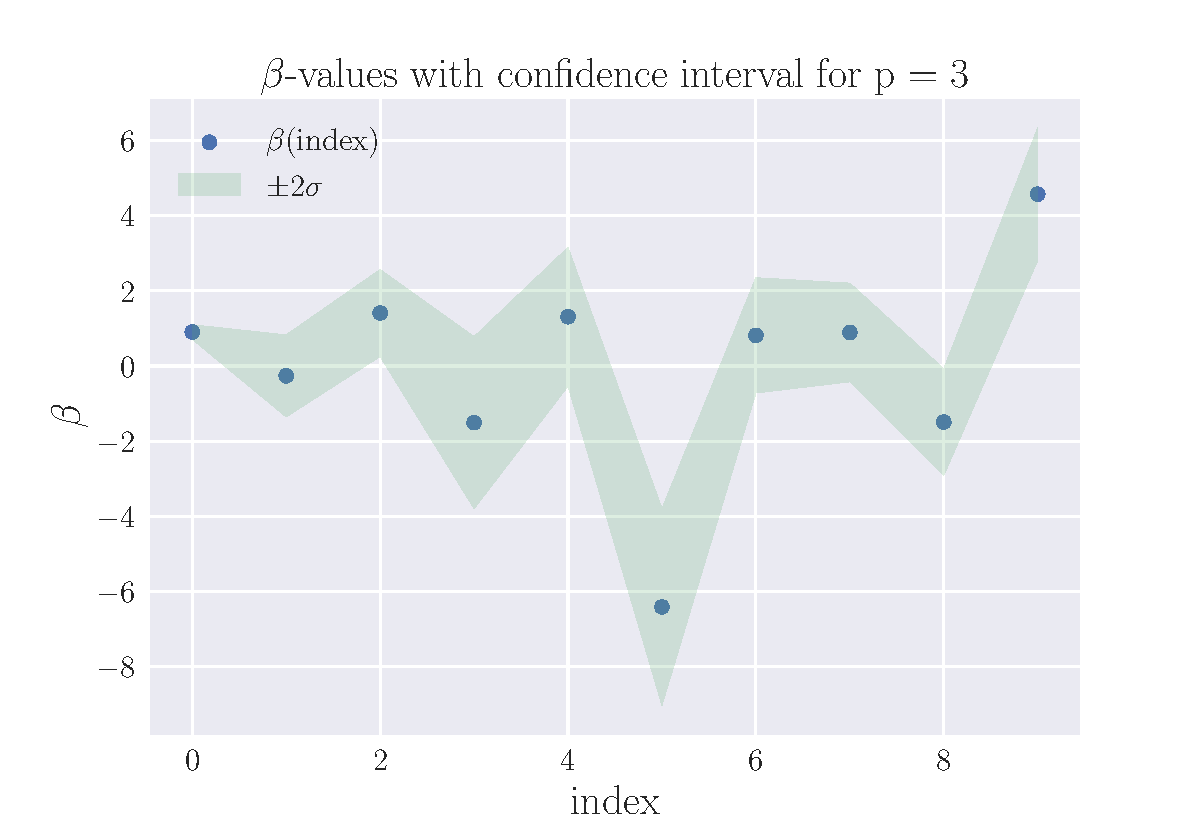
\includegraphics[width=\linewidth]{Var_OLS_poldeg_3.pdf}
	\endminipage\hfill
	\minipage{0.49\textwidth}
	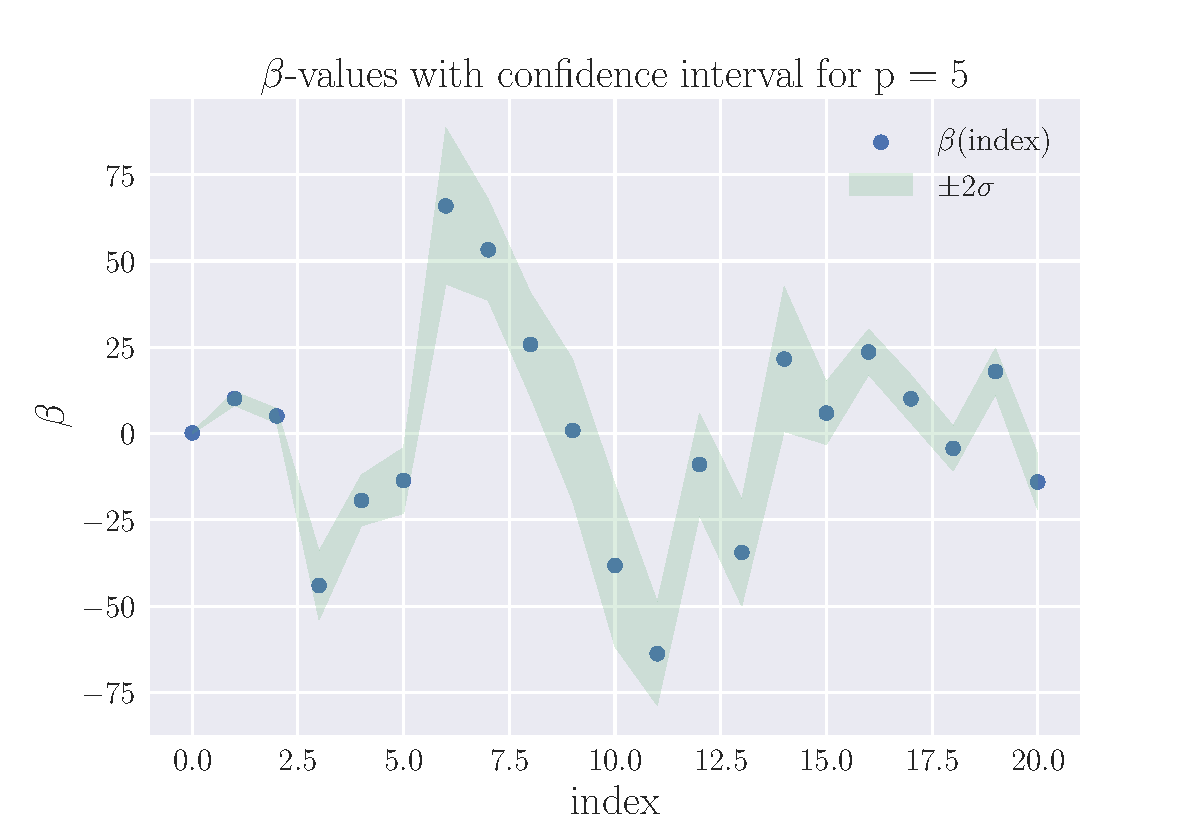
\includegraphics[width=\linewidth]{Var_OLS_poldeg_5.pdf}
	\endminipage\hfill
	\minipage{0.49\textwidth}
	\caption{Here we have plotted the ideal parameters, for different polynomial degrees and with the confidence intervals. Top left figure has polynomial degree $p = 1$, top right $p = 3$ and bottom left $p = 5$. All the plots are of $\boldsymbol{\beta}$ as a function of the index in the vector. The confidence interval is $\pm 2\boldsymbol{\sigma}(\boldsymbol{\hat{\beta}}_{j})$, where $\boldsymbol{\sigma}(\boldsymbol{\hat{\beta}}_{j})$ is given by equation \eqref{eq:var_OLS}.} \label{fig:var_beta}
	\endminipage
\end{figure}
We see in figure \ref{fig:var_beta} that the variance increases as a function of $p$. This is expected because we should get overfitting for higher polynomial degrees. For larger $p$ we also have more parameters to tune. This means that a change in one, could be compensated for by tuning the other parameters in the vicinity. We can see the result of this in the bottom left plot in figure \ref{fig:var_beta}. We observe a large variance in the middle, where we have a high density of parameters, and a lower variance on the edges. One also notices an comparatively low variance for the first parameter $\beta_0$, because the fixed intercept.


\section*{Exercise 2: Bias-variance trade-off and bootstrapping}

Here we want to evaluate OLS using bootstrapping as a resampling technique. Bootstrap is a way of simulating having more data than you actually have, by reusing the same data. Lets say you have $N$ datapoints, then you would draw $N$-times, placing back the datapoint each time. Then perform the regression analysis, and repeat this process $B$-times. By placing back the datapoints, you would in many cases use the same datapoint several times.

Now, with bootstrapping, we want to take a look at when we get overfitting. It is common to see overfitting when we have a high polynomial degree ($p_\text{max}$) compared to the number of datapoints. Thus in figure \ref{fig:OLS_overfitting} we have plotted the test and train MSE for $p_\text{max} = 20$, using $B=90$ resampling iterations. The left plot shows an indication of overfitting at polynomial degree $p = 9$. Thus on the right hand plot we have displayed the MSE for $p_\text{max} = 10$, and as expected we see overfitting at $p=9$. One unexpected result is the sharp increase and decrease in MSE. This indicates that our model is much better for some polynomial degrees than others. The sharp fluctuations can be explained by the surge in complexity from one polynomial degree to the next. This is displayed in figure \ref{fig:var_beta}, when we increase the polynomial degree by two, the number of parameters more than double.

\begin{figure}[H]
	\minipage{0.49\textwidth}
	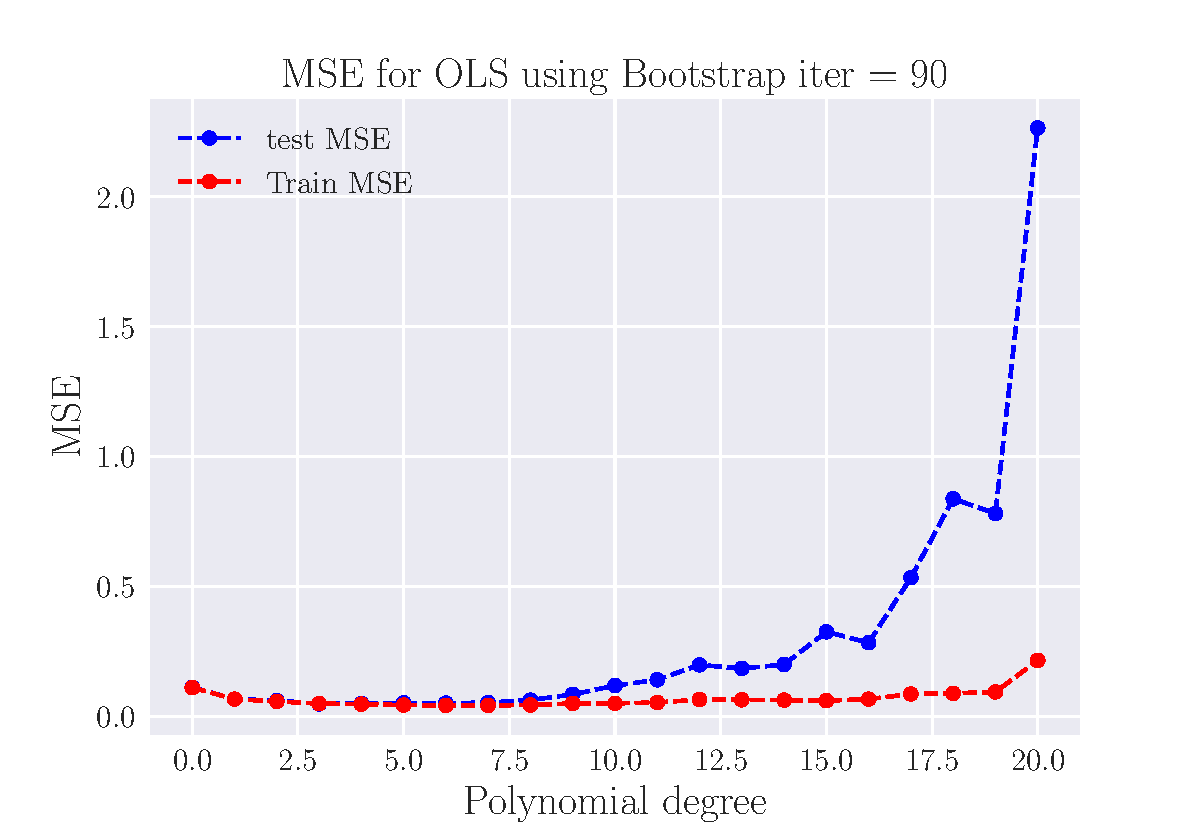
\includegraphics[width=\linewidth]{MSE_OLS_n30_eps02_pol20_Bootstrap_re90.pdf}
	\endminipage\hfill
	\minipage{0.49\textwidth}
	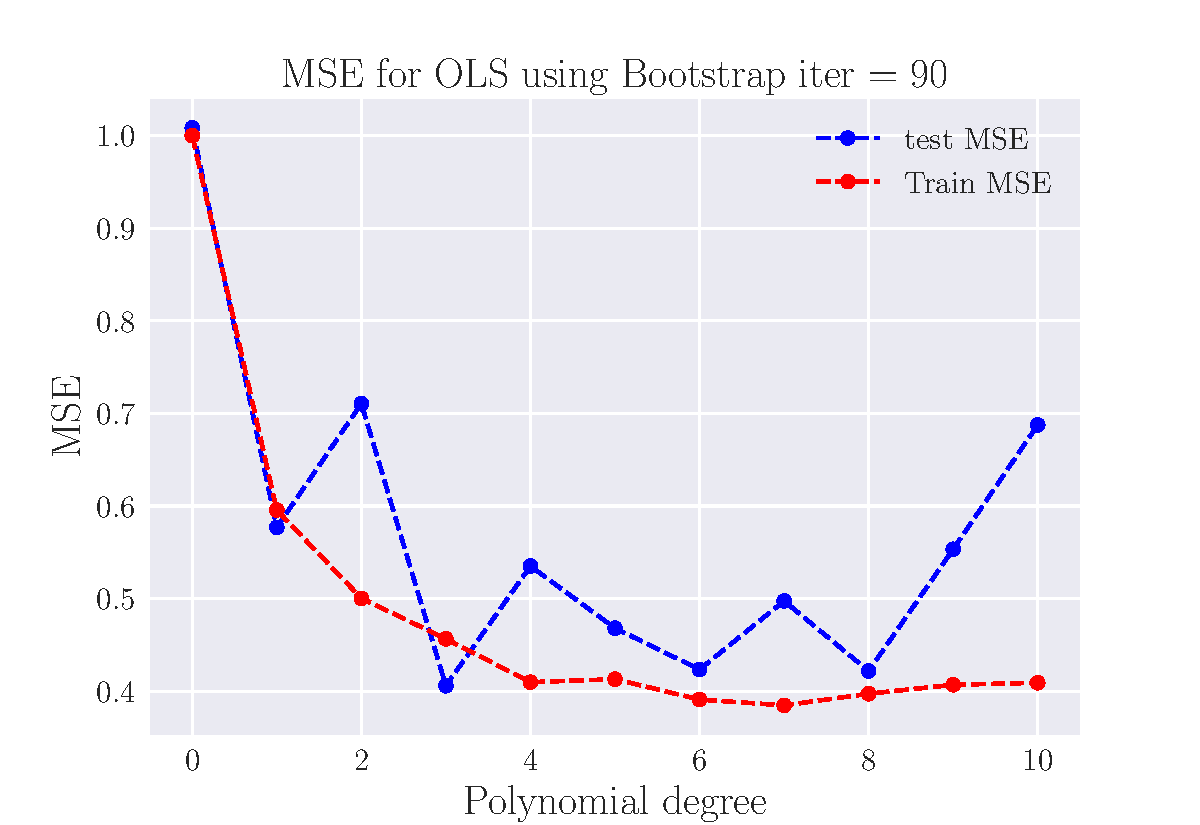
\includegraphics[width=\linewidth]{MSE_OLS_n30_eps02_pol10_Bootstrap_re90.pdf}
	\endminipage
	\caption{Overfitting, høyre med støy, venstre uten støy.}\label{fig:OLS_overfitting}
\end{figure}

Before we take a look at bias variance trade-off, we will derive the expressions. With our data model given in equation \eqref{eq:z_true_data} we find our model by considering the cost function, given as
\begin{align*}
  C(\bm{\beta}) &= \frac{1}{N} \sum_{i=0}^{N-1} (z_i - \tilde{z}_i)^2 = \mathbb{E}[(\mathbf{z}-\mathbf{\tilde{z}})^2]
\end{align*}
where $\mathbb{E}$ is the expected value. % Sample value

We can show that this can be written as \footnote{The derivation is given in Appendix \ref{Apx:BVT}}

\begin{align}
\label{eq:bias_var_tradeoff}
  \mathbb{E}[(\mathbf{z}-\mathbf{\tilde{z}})^2] &= \frac{1}{N}\sum_i (f_i - \expz)^2 + \frac{1}{N}\sum_i (\tilde{z}_i - \expz)^2 + \sigma^2
\end{align}
where $f_i$ is the true data value at point $i$.

In equation \eqref{eq:bias_var_tradeoff} the first term represents the square of the bias, the second term represents the variance while the last term represents the variance of the irreducable error $\epsilon$. When performing linear regression the variance is a measurement on how much our model changes with different training sets. High variance will therefore occur if a different training set resulted in very different values of the individual estimators, $\bm{\beta}$. This will be the case for overfitting when our model is essentially trying to reproduce variations from the noise. The bias provides information about the difference between our model and the true data values. If our model is missing out on underlying structures in our data we would get a high bias. High bias will thus be the case for an underfitted model. Our goal is therefore to minimize the bias and variance in our model.

Using equation \eqref{eq:bias_var_tradeoff} we can plot the bias, variance and MSE for the test and train data, using the bootstrap method. For both datasets we expect the bias and MSE to start high and variance to start low. For the train data we should get a strictly better fit for higher polynomial degree, making both the bias and MSE to decrease. For the testing data however, when we start to see overfitting (around $p=9$) variance and error should increase, while bias stays low. In figure \ref{fig:BV_OLS} we have plotted bias, variance and MSE for the test and train data, using $B = 90$ resampling iterations. Because we expected to see overfitting at around $p=9$ we plotted for $p_\text{max} = 10$.

\begin{figure}[H]
	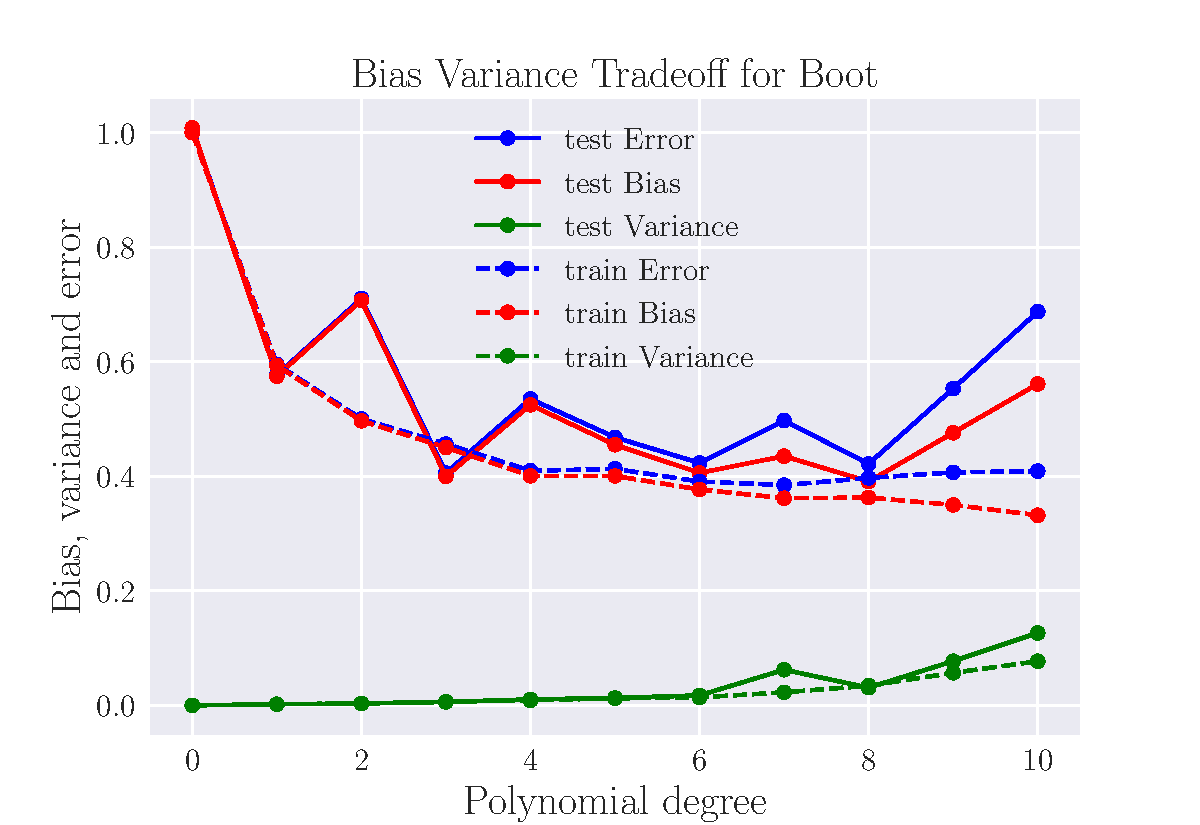
\includegraphics[width=\linewidth]{BVT_OLS_n30_eps0_2.pdf}
	\caption{Here we have plotted the bias, variance and MSE for the test and train data. The $x$-axis shows the polynomial degree, and the $y$-axis indicates the bias, variance and MSE. The dotted lines are for the train data and solid lines are the test data.}\label{fig:BV_OLS}
\end{figure}

As expected we se an increase in MSE and variance for the test data, when we start overfitting. The bias does not act completely as expected. It does decrease in the beginning, however it starts increasing with the MSE again at around $p = 8$. This however could be due to the sensitive nature of bootstrapping. As we saw in \ref{Apx:testing_BVT}, bias variance analysis with bootstrapping is very sensitive to the number of resampling iterations $B$, and gives unexpected results because of it. One thing we also saw in the overfitting experiment (figure \ref{fig:OLS_overfitting}) is the sharp increase and decrease for specific polynomial degrees. Taking all of this into account, the optimal fit that minimizes bias, variance and MSE for OLS is $p=6$.

\section*{Exercise 3: Cross-validation as resampling technique, adding more complexity}

Here we have implemented cross-validation as the resampling technique. This works by first shuffling the data randomly, then split the data into $k$ different groups. We can then decide on one group to be the test-data and perform linear regression on the rest. After that we can calculate the MSE, and repeat this process $k$-times. The final MSE would then be the mean MSE, after all the iterations. In figure \ref{fig:CV_OLS} we have done this, trying for $k = [5,7,10]$.

\begin{figure}[H]
	\minipage{0.49\textwidth}
	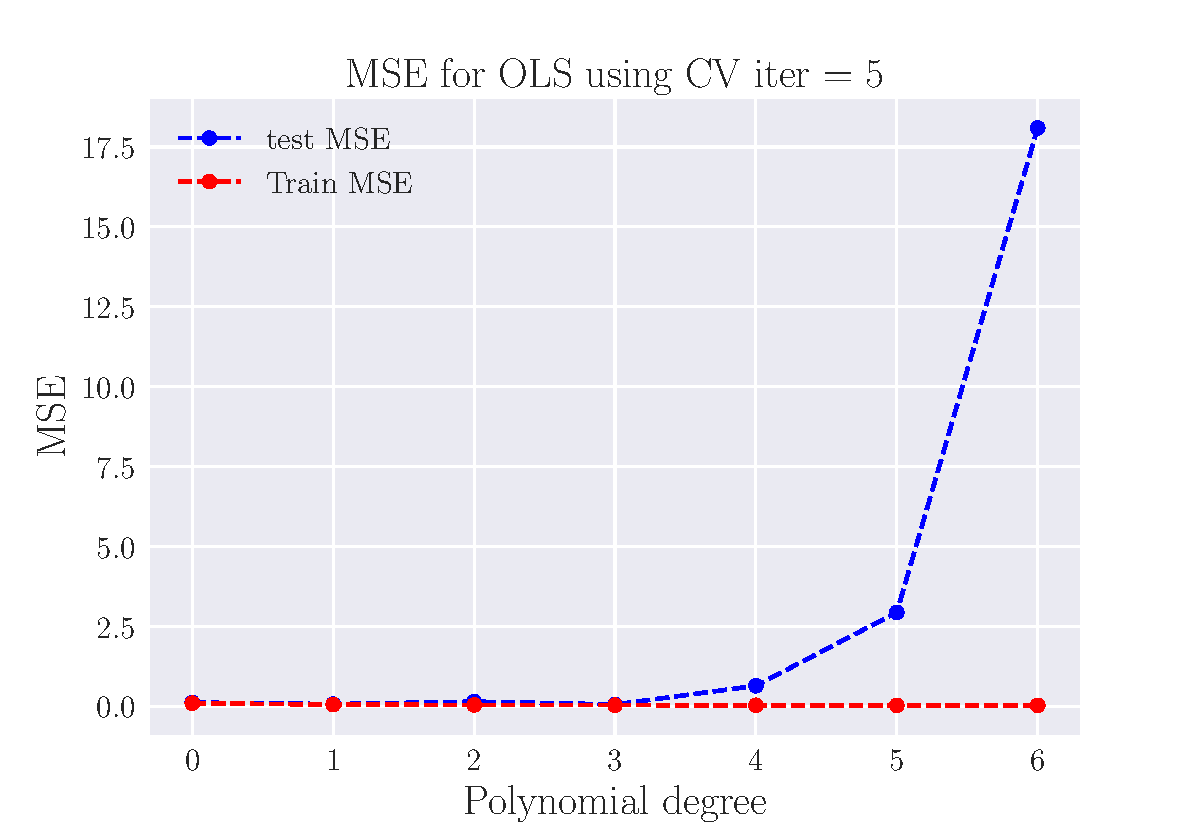
\includegraphics[width=\linewidth]{MSE_OLS_n30_eps02_pol6_CV_re5.pdf}
	\endminipage\hfill
	\minipage{0.49\textwidth}
	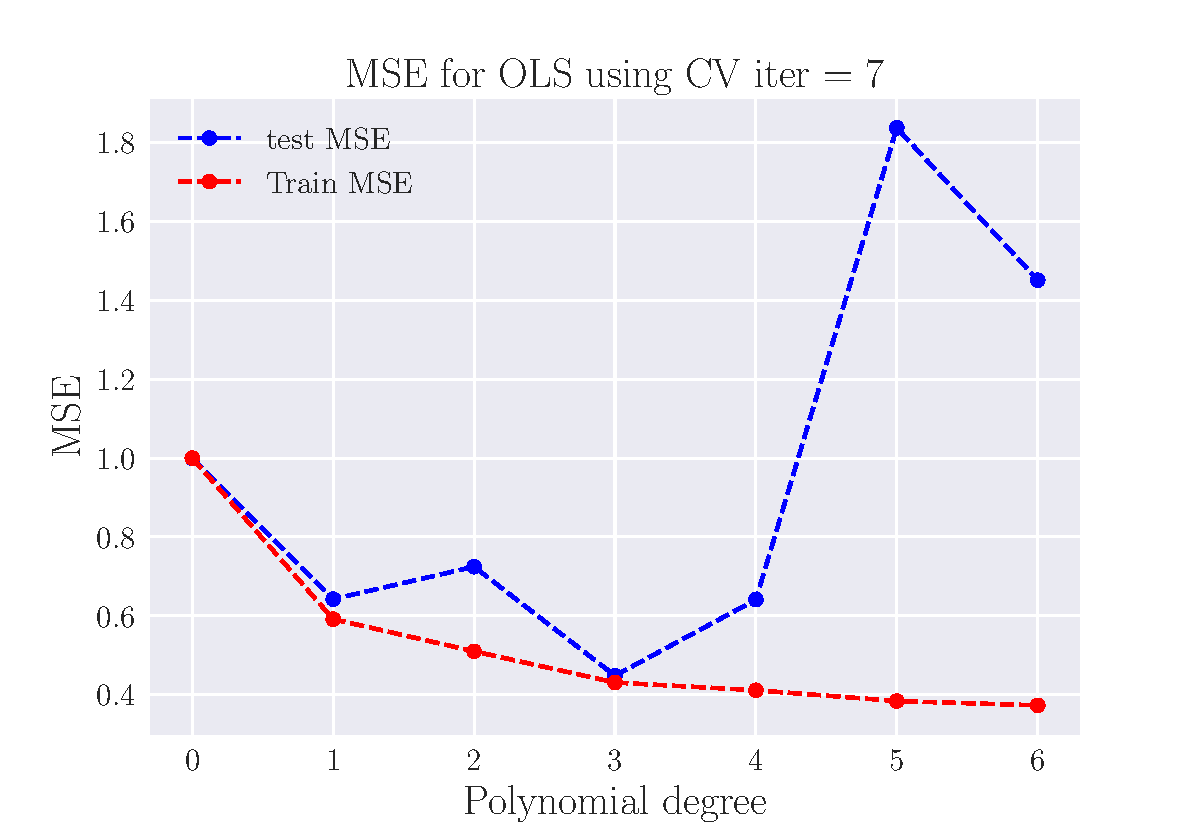
\includegraphics[width=\linewidth]{MSE_OLS_n30_eps02_pol6_CV_re7.pdf}
	\endminipage\hfill
	\minipage{0.49\textwidth}
	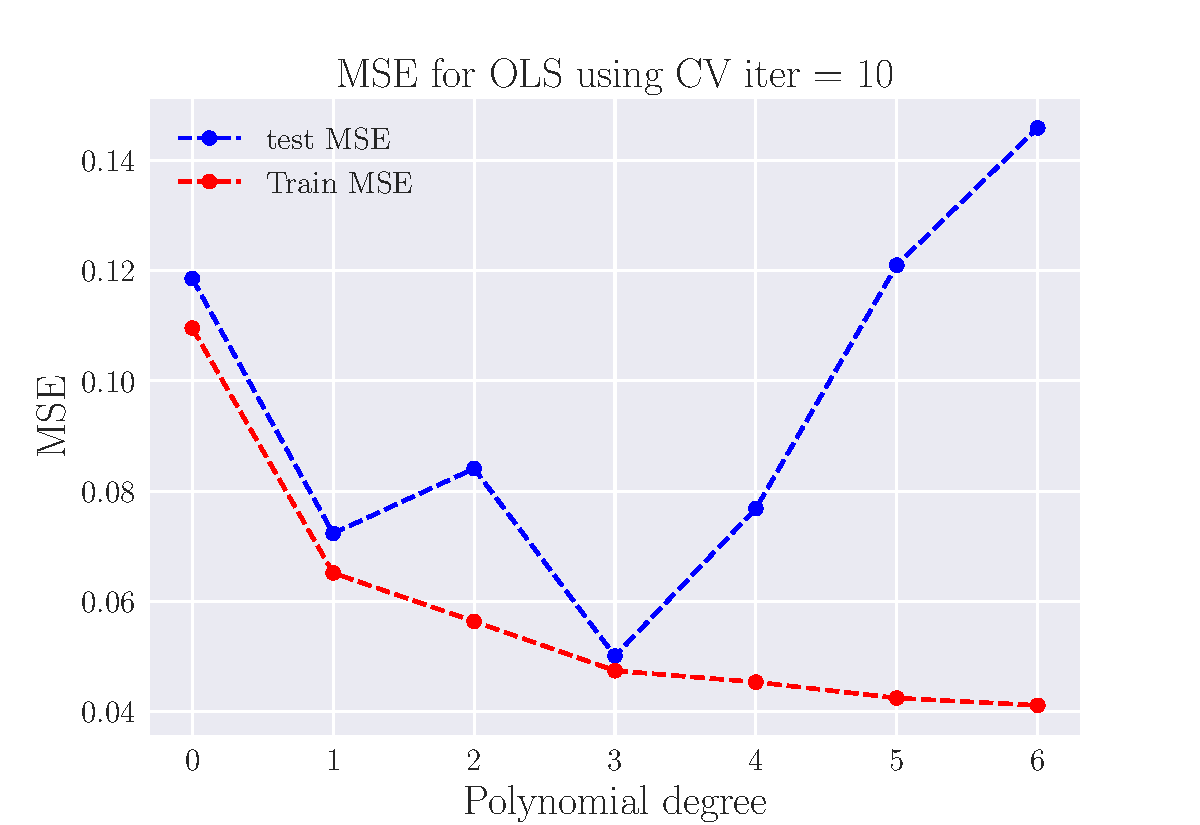
\includegraphics[width=\linewidth]{MSE_OLS_n30_eps02_pol6_CV_re10.pdf}
	\endminipage\hfill
	\minipage{0.49\textwidth}
	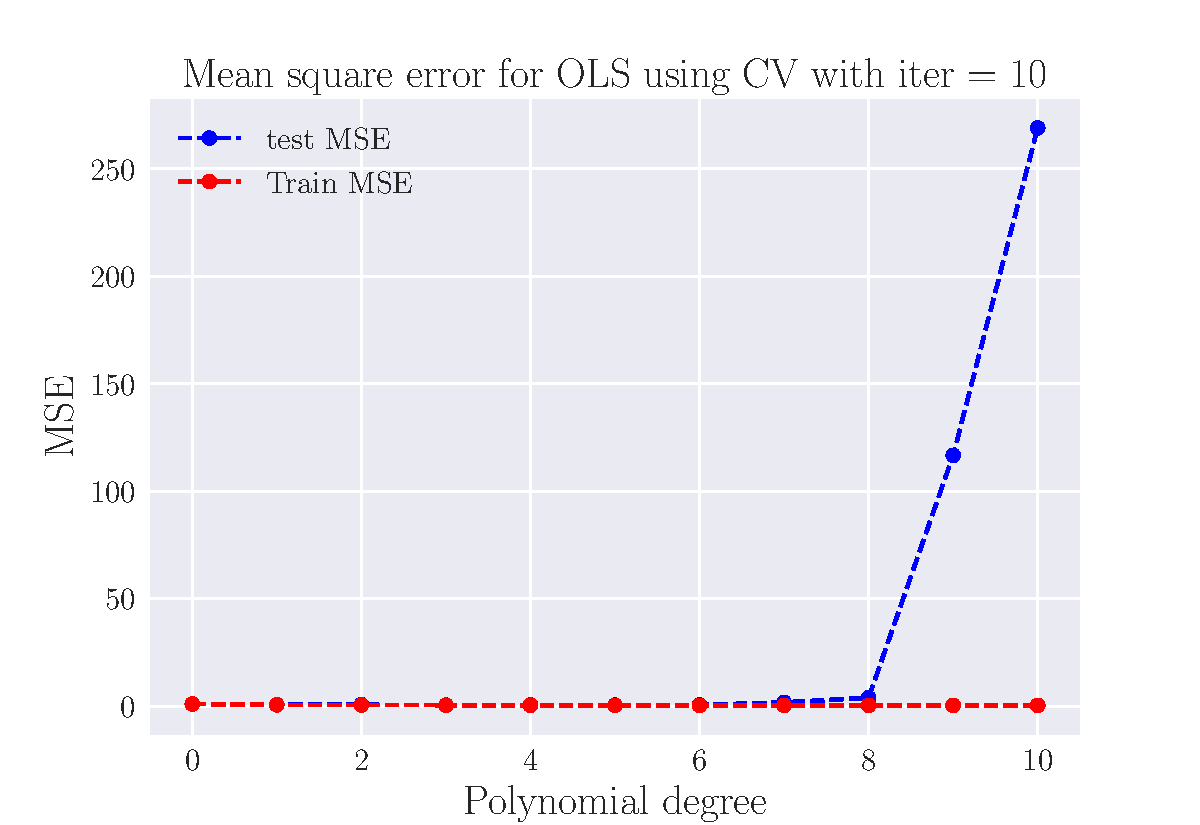
\includegraphics[width=\linewidth]{MSE_OLS_n30_eps02_pol10_CV_re10.pdf}
	\endminipage
	\caption{Here we have plotted the MSE when performing cross-validation as the resampling technique. On the $x$-axis we have polynomial degree, and MSE on the $y$-axis. The top left, right and bottom left figures are with $k=[5, 7, 10]$ iterations respectively. The bottom left plot is to illustrate the diverging MSE for higher polynomial degree, which we see irregardless of iteration-number.} \label{fig:CV_OLS}
\end{figure}

When bootstrapping we saw overfitting at around $p=6$. Looking at the plots in figure \ref{fig:CV_OLS} there seems to be consistent overfitting at around $p=3$. In the bottom right plot we have plotted for higher polynomials to illustrate that this error does not decrease for higher $p$. This does not depend on the number of resampling iterations. We see no obvious reason that the overfitting should start sooner compared to bootstrapping, and thus ground it in random fluctuations. We have consistently seen large variation in results based on number of resampling, and the random seed used when producing the results. Another interesting result is that a higher number of resampling iterations seems to decrease the overfitting effects. This coincide with the analysis on early overfitting. Having a larger number of resampling iterations should dampen the odd effects due to randomness.

\section*{Exercise 4: Ridge Regression on the Franke function with resampling}
In some cases, it might happen that the matrix $\mathbf{X}^T\mathbf{X}$ is singular, such that it is non-invertible. This is the case if some of the independent variables are highly correlated. Then OLS will not work, see \eqref{eq:OLS_beta}. However, by subtracting a small number $\lambda$ from the diagonal, the matrix is no longer singular. This is called Ridge regression. The optimal parameters $\boldsymbol{\hat\beta}$ are given by
\begin{equation}
	\boldsymbol{\hat{\beta}} = (X^TX-\lambda I)X^T\vc{z},
\end{equation}
where $I$ is  the identity matrix. The parameter $\lambda$ can take any value, so finding the optimal is paramount. This is done by running the regression for many different values of $\lambda$ and choosing the one giving the best results. Now we want to perform the same bootstrap analysis as we did for OLS, using Ridge. Here we also take a look at when we have overfitting, for different values of $\lambda$ and with bootstrap.

\begin{figure}[H]
	\minipage{0.49\textwidth}
	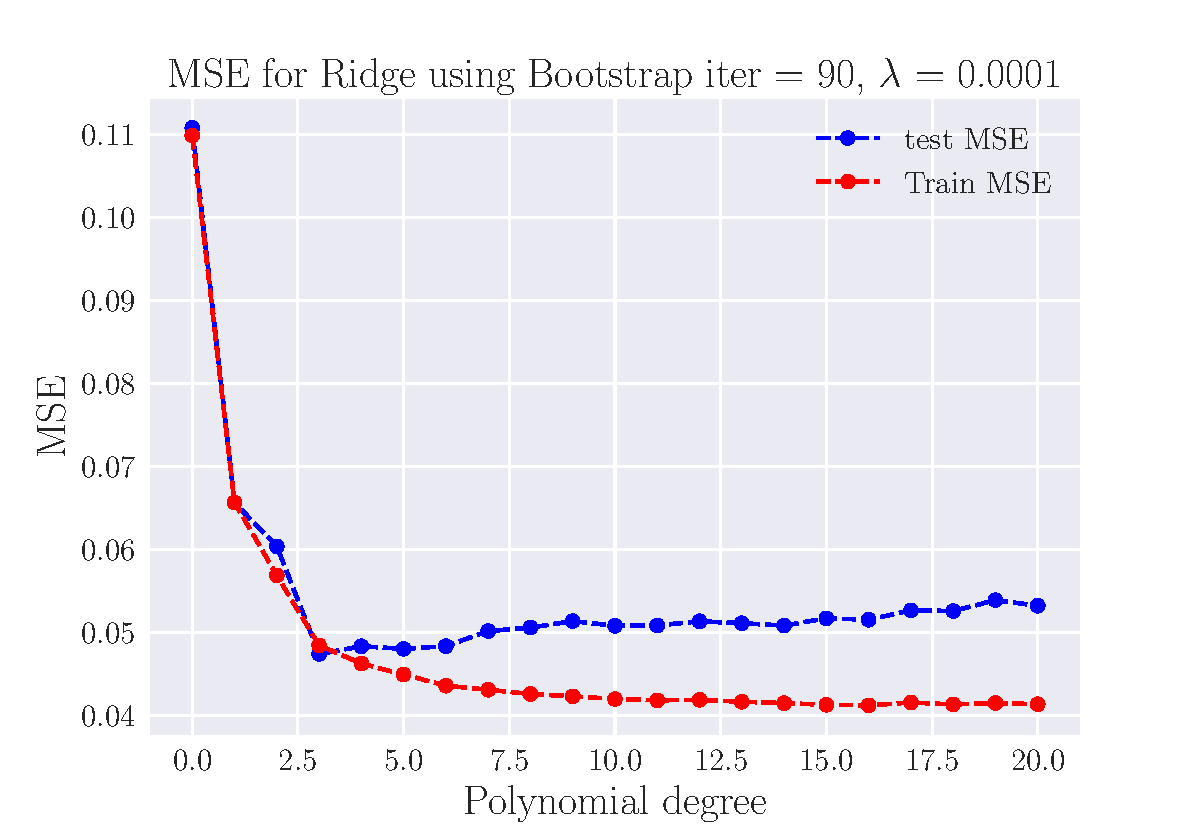
\includegraphics[width=\linewidth]{MSE_Ridge_n30_eps02_pol20_Bootstrap_re90_lam_0_0001.pdf}
	\endminipage\hfill
	\minipage{0.49\textwidth}
	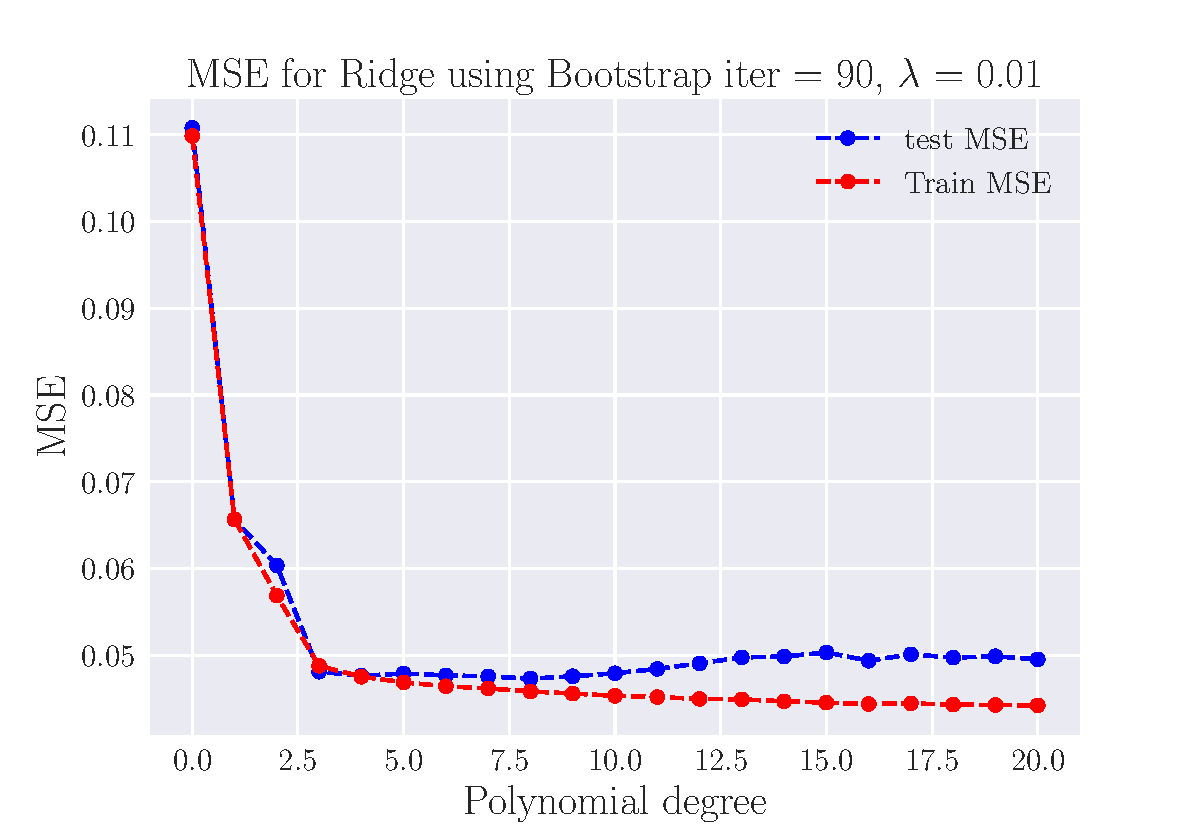
\includegraphics[width=\linewidth]{MSE_Ridge_n30_eps02_pol20_Bootstrap_re90_lam_0_01.pdf}
	\endminipage\hfill
	\minipage{0.49\textwidth}
	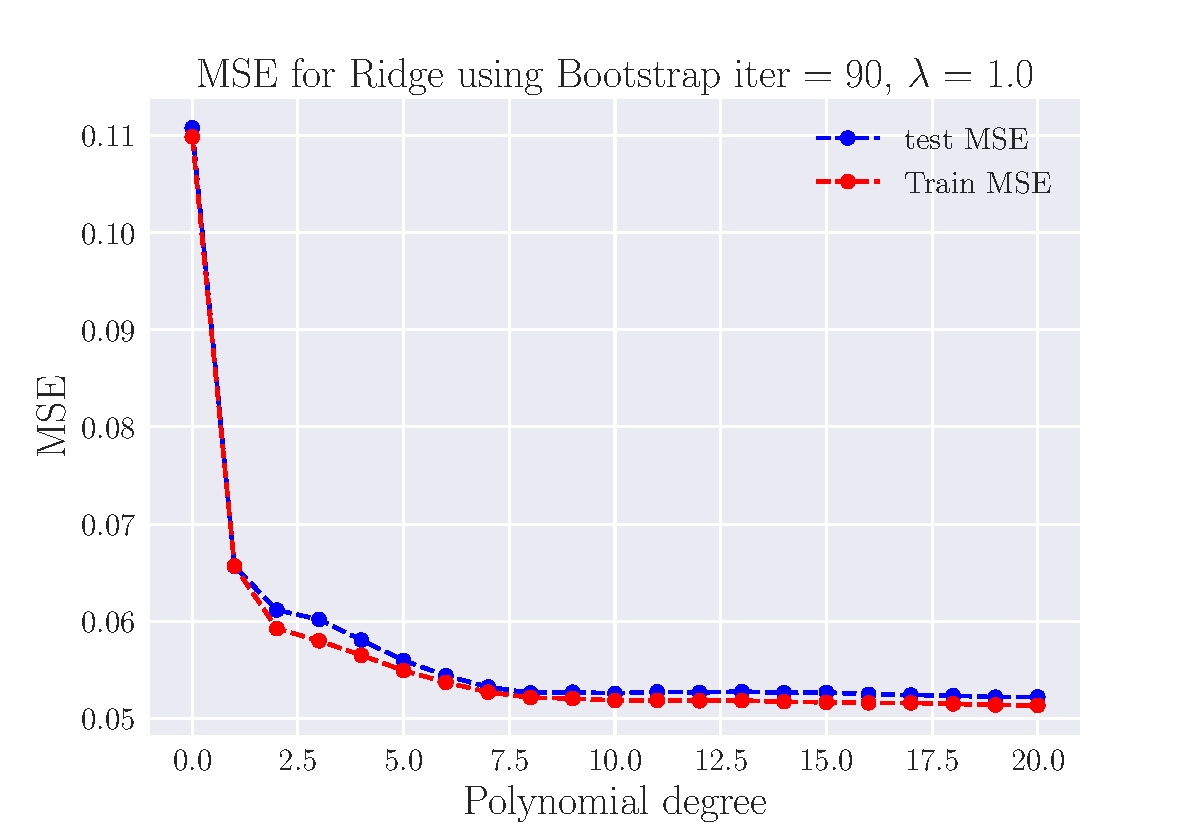
\includegraphics[width=\linewidth]{MSE_Ridge_n30_eps02_pol20_Bootstrap_re90_lam_1_0.pdf}
	\endminipage\hfill
	\minipage{0.49\textwidth}
	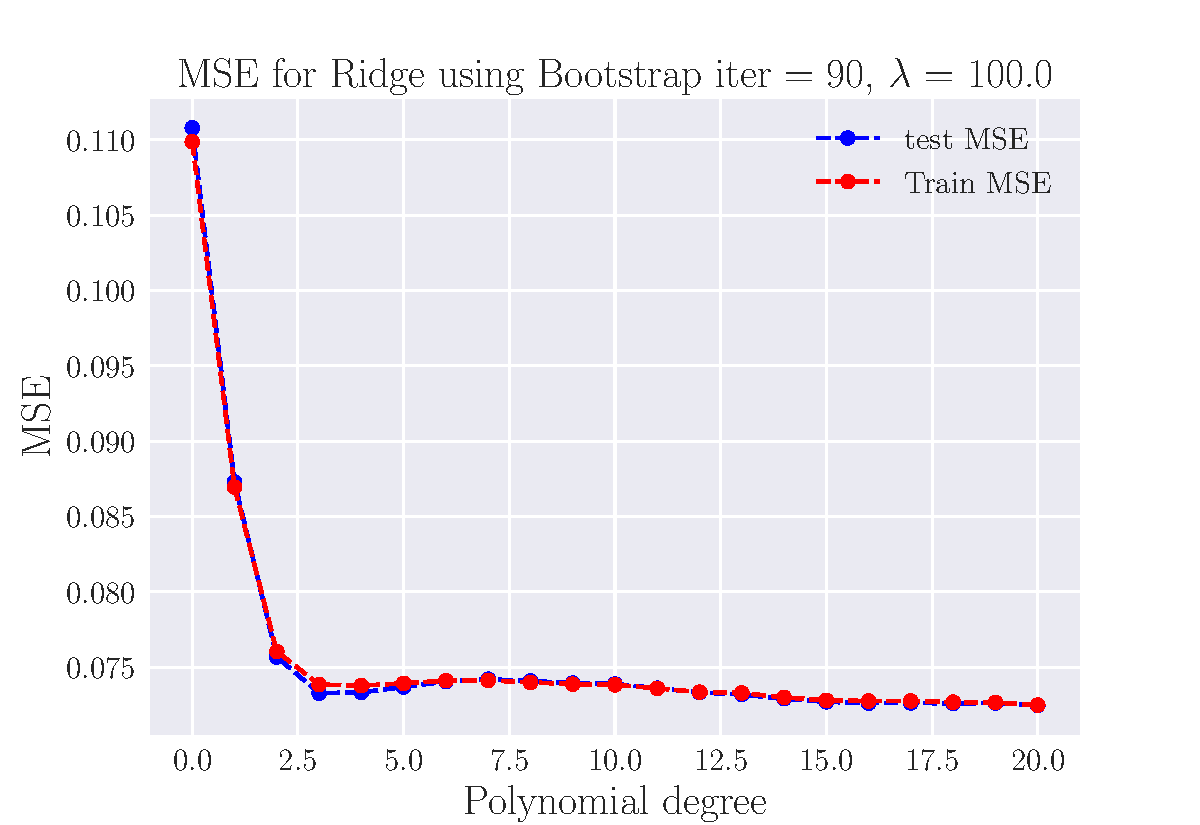
\includegraphics[width=\linewidth]{MSE_Ridge_n30_eps02_pol20_Bootstrap_re90_lam_100_0.pdf}
	\endminipage
	\caption{Plot av MSE med BOOT for Ridge} \label{fig:Ridge_overfitting}
\end{figure}

\begin{figure}[H]
	\minipage{0.49\textwidth}
	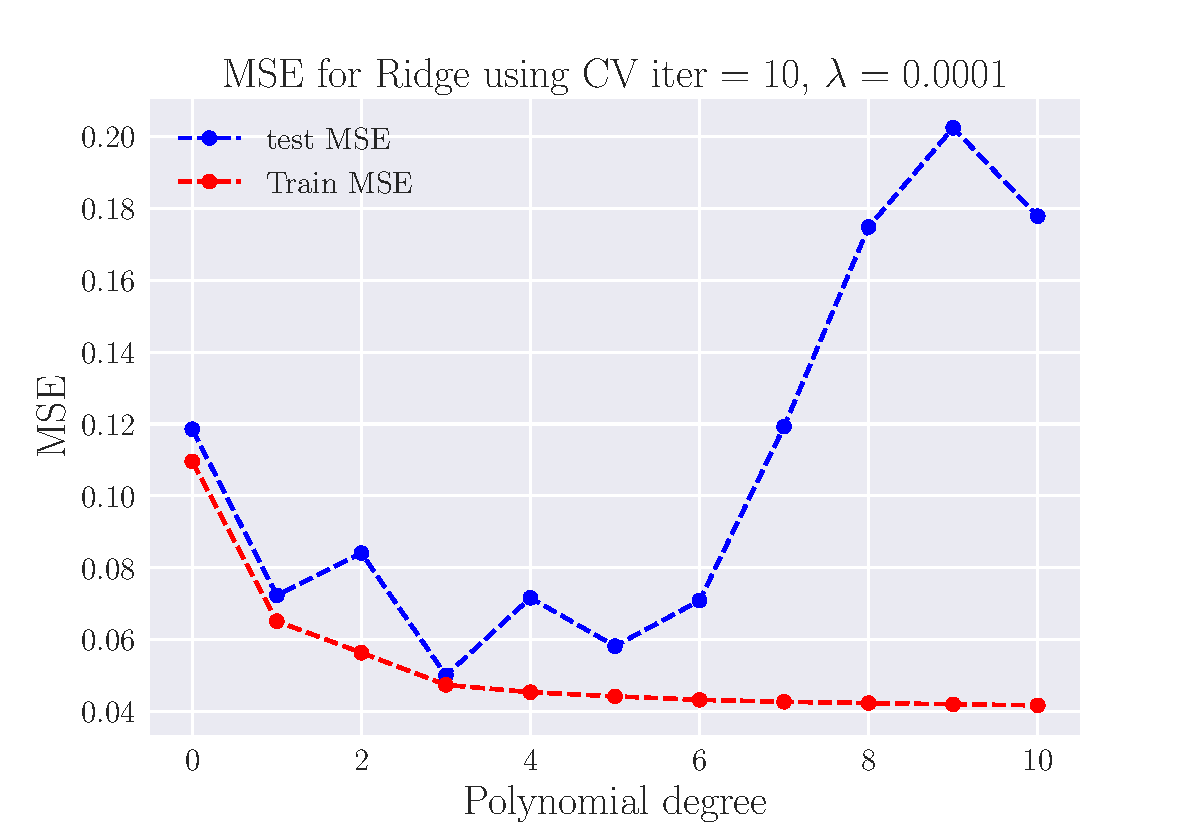
\includegraphics[width=\linewidth]{MSE_Ridge_n30_eps02_pol10_CV_re10_lam_0_0001.pdf}
	\endminipage\hfill
	\minipage{0.49\textwidth}
	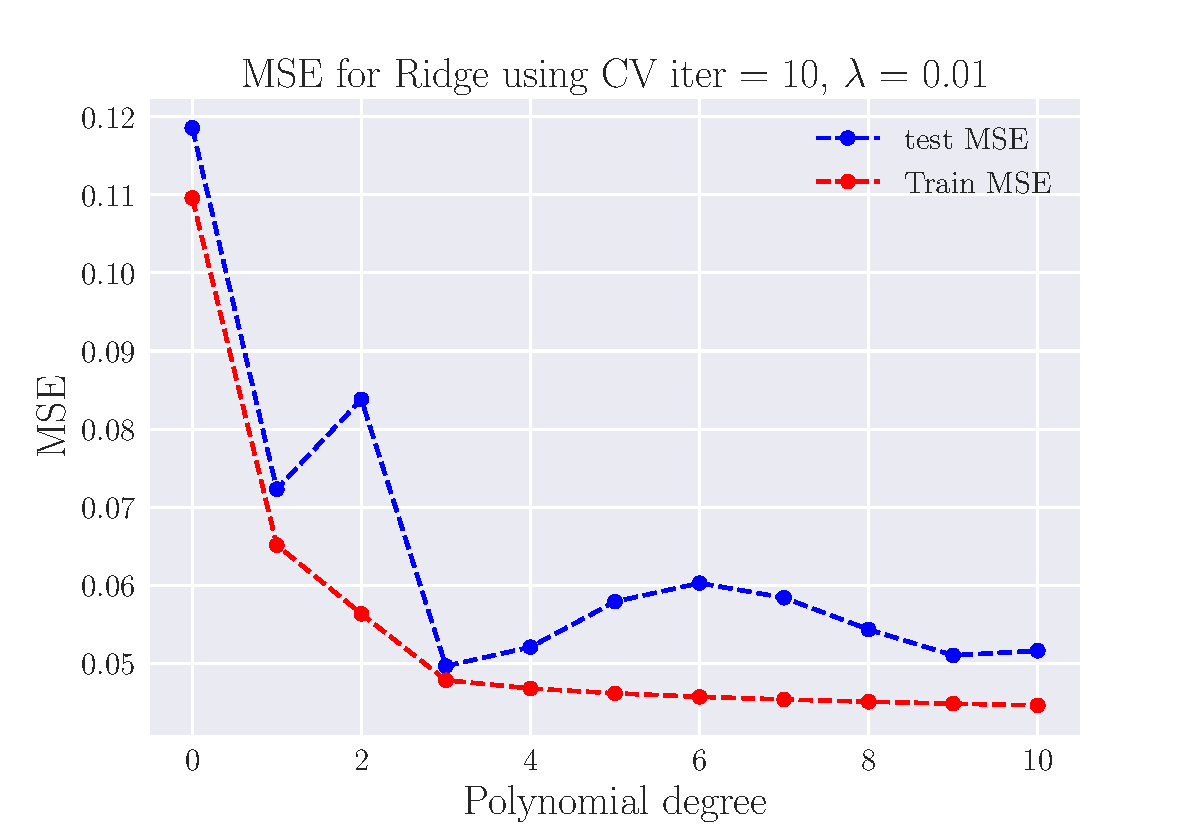
\includegraphics[width=\linewidth]{MSE_Ridge_n30_eps02_pol10_CV_re10_lam_0_01.pdf}
	\endminipage\hfill
	\minipage{0.49\textwidth}
	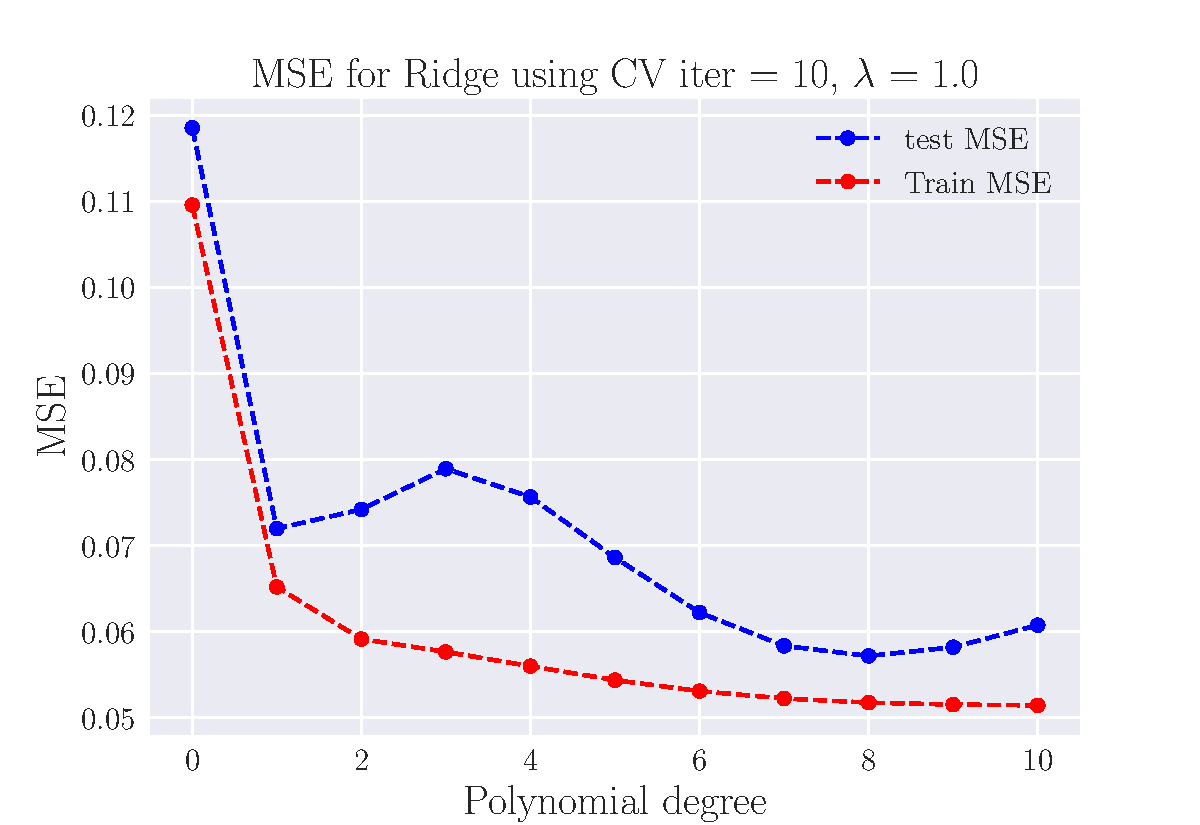
\includegraphics[width=\linewidth]{MSE_Ridge_n30_eps02_pol10_CV_re10_lam_1_0.pdf}
	\endminipage\hfill
	\minipage{0.49\textwidth}
	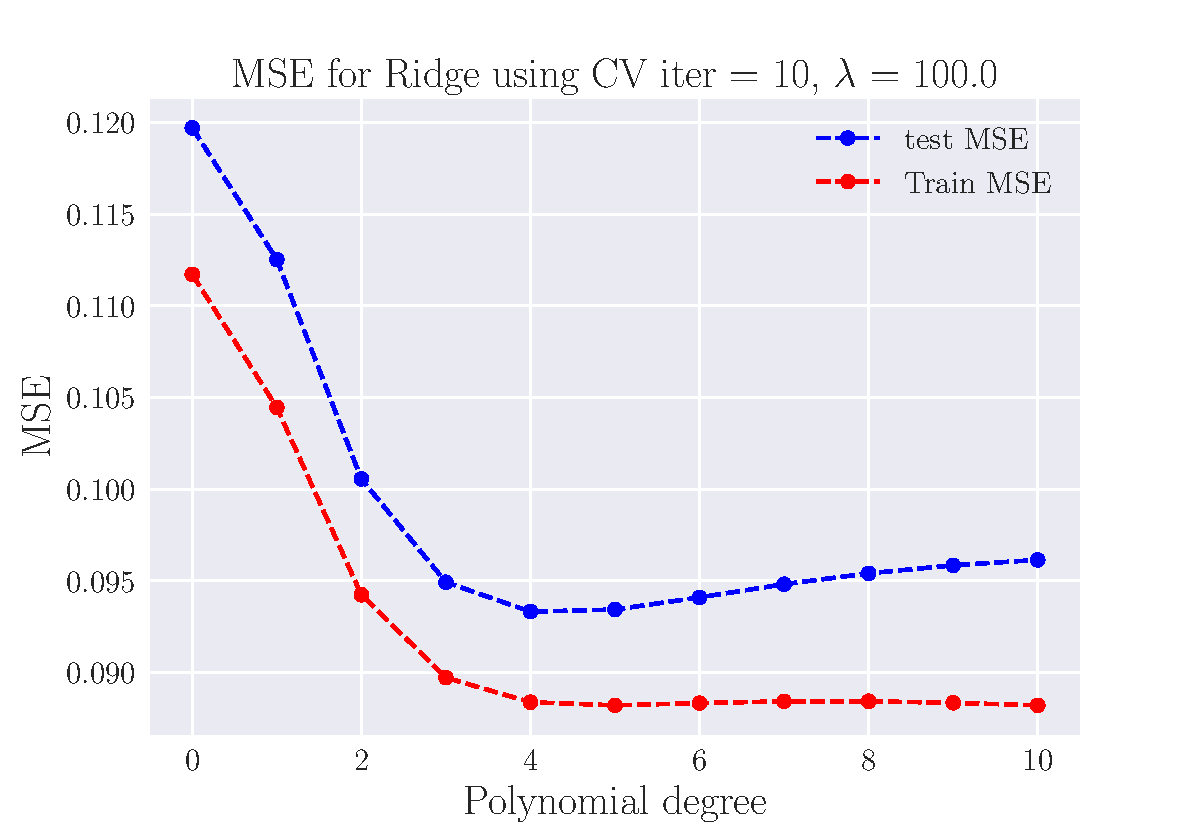
\includegraphics[width=\linewidth]{MSE_Ridge_n30_eps02_pol10_CV_re10_lam_100_0.pdf}
	\endminipage
	\caption{Plot av MSE med BOOT for Ridge} \label{fig:Ridge_CV}
\end{figure}


\section*{Exercise 5: Lasso regression on the Franke function with resampling}


\section*{Exercise 6: Analysis of real data}

Having used our data analysis methods to study the Franke function we will now move on to study data from the real world. We will consider terrain data from Norway !HVOR?!. The terrain data we consider is shown in figure \ref{fig:terrain_raw}.

\begin{figure}[H]
  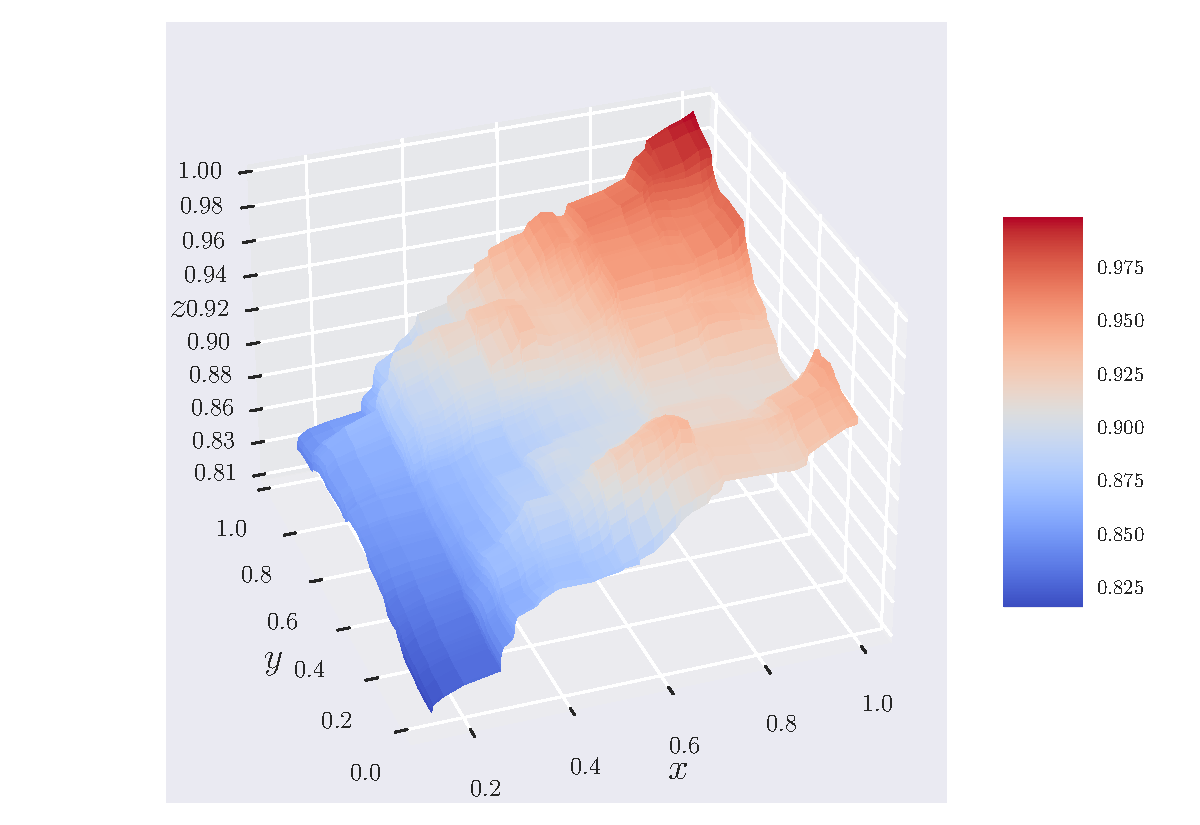
\includegraphics[width=\linewidth]{SRTM_rawdata_n50.pdf}
  \caption{Raw terrain data}
  \label{fig:terrain_raw}
\end{figure}

We begin by studying the mean squared error with OLS-regression, where we use the bootstrap resampling method with $50$ resampling iterations. For our original data set with $50$ data points in both directions, we consider polynomials up to a maximum degree of $25$. The resulting mean squared error is shown on the left panel in figure \ref{fig:terrain_OLS_MSE_bootstrap} with a logarithmic y-axis. Using a data set with $50\cross50$ data points yields a little noticeable change in the mean squared error, but we see a potential overfitting occuring for $P>15$. To see that we get overfitting for the terrain data eventually, we plot the mean squared error for the same resampling method, but with $n=10$ points in each direction up to a polynomial degree of $P=10$, shown on the right panel in figure \ref{fig:terrain_OLS_MSE_bootstrap}. Here, we can see an evident overfitting starting to occur for polynomial degrees greater than $6$.

\begin{figure}[H]
  \minipage{0.49\textwidth}
  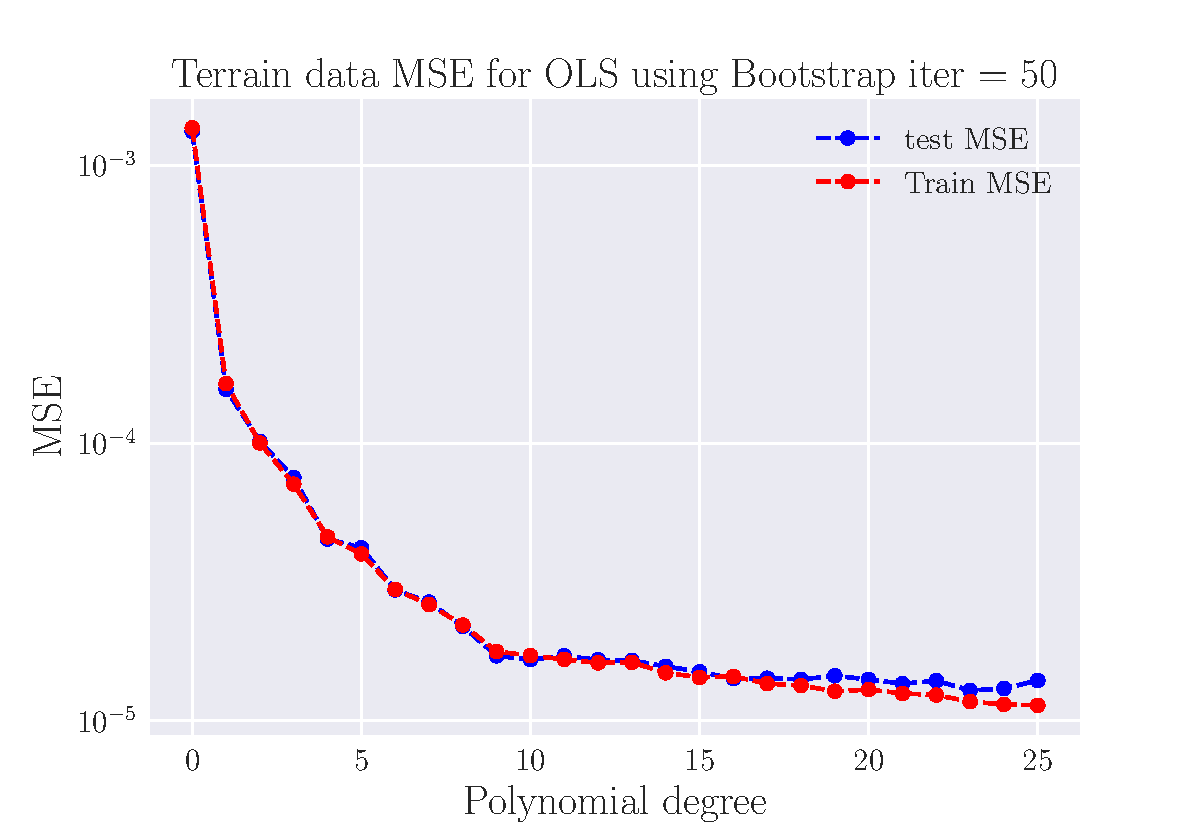
\includegraphics[width=\linewidth]{SRTM_MSE_OLS_n50_pol25_Bootstrap_re50_log.pdf}
  \endminipage\hfill
  \minipage{0.49\textwidth}
  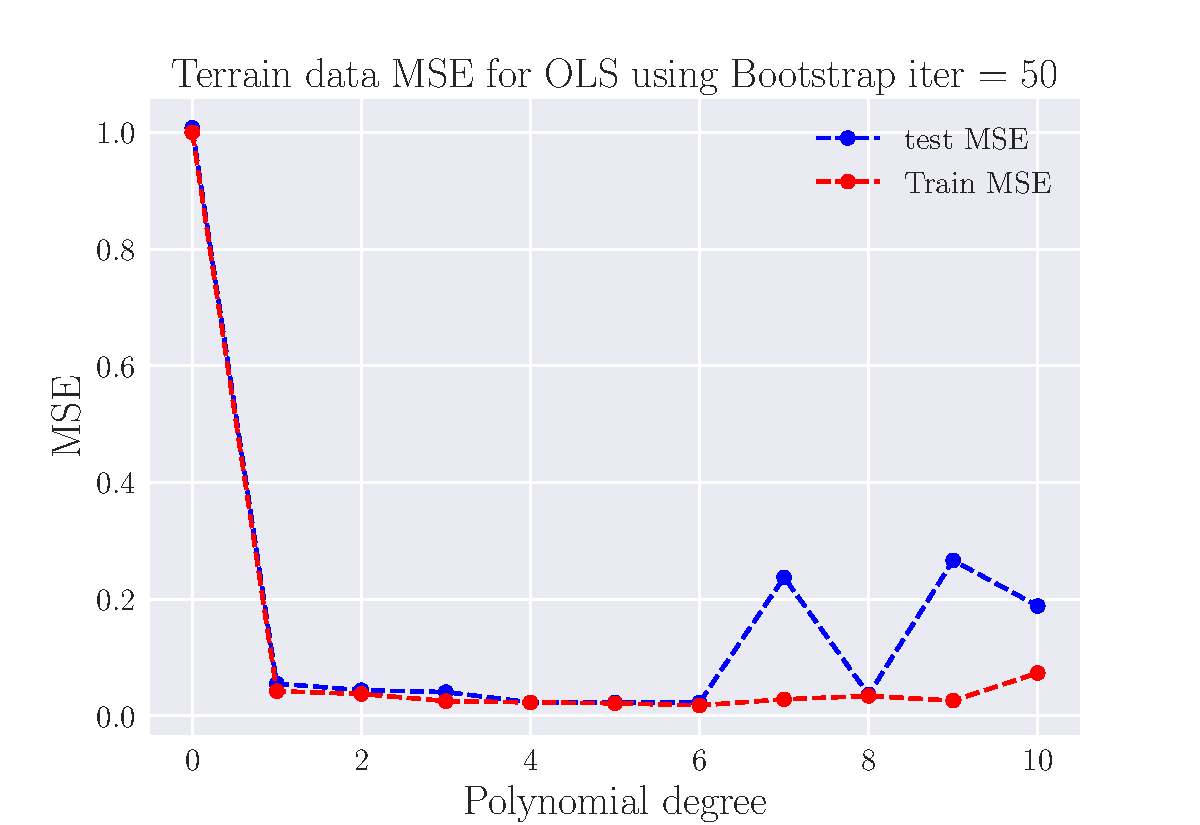
\includegraphics[width=\linewidth]{SRTM_MSE_OLS_n15_pol10_Bootstrap_re50.pdf}
  \endminipage
  \caption{n50 log til venstre. n15 til høyre}
  \label{fig:terrain_OLS_MSE_bootstrap}
\end{figure}

As a simple sanity check, we plot the result of our fits for different polynomial degrees, which we can compare to the original data from figure \ref{fig:terrain_raw}. To capture the complexity of our data set, we consider four polynomial degrees, using $P\in[10,\,20,\,30,\,50]$, where the first two are shown in the upper left and right panel of figure \ref{fig:terrain_fit}, respectively, while the latter two in the bottom left and right panel of the same figure, respectively.

\begin{figure}[H]
	\minipage{0.49\textwidth}
	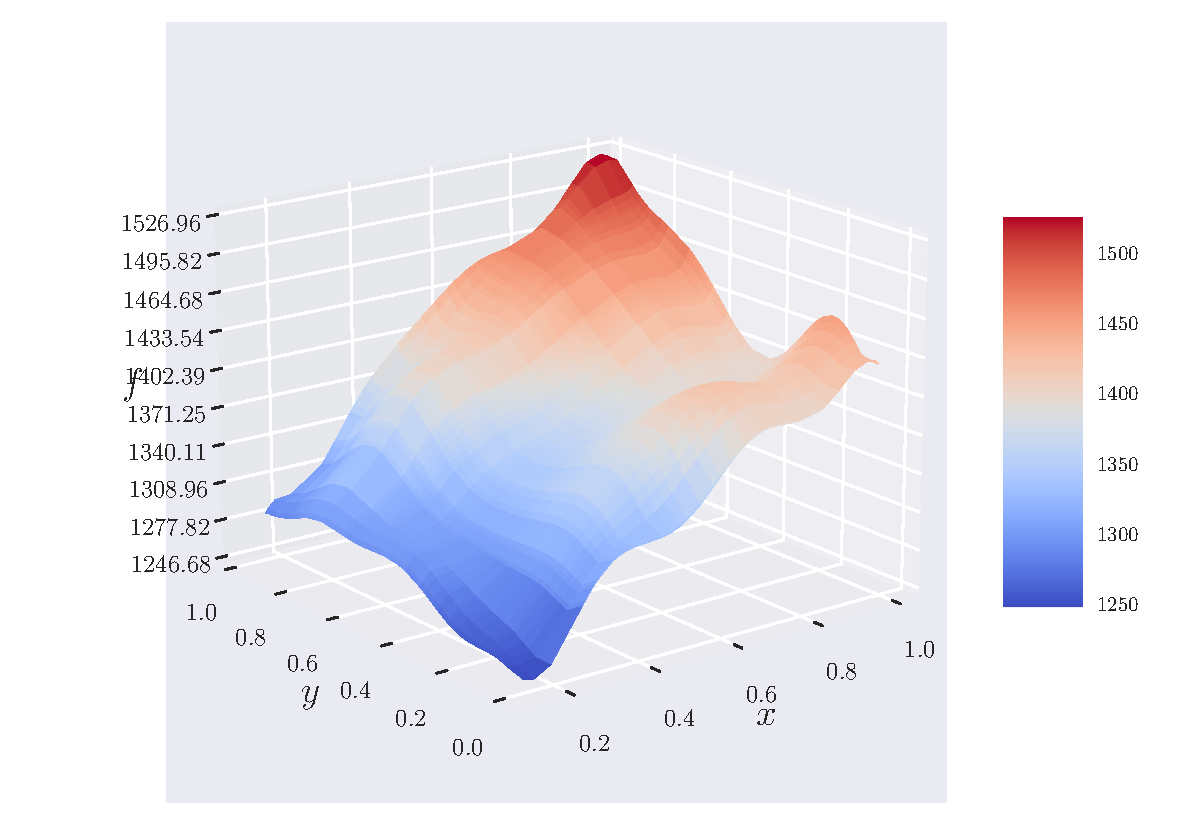
\includegraphics[width=\linewidth]{SRTM_prediction_p10.pdf}
	\endminipage\hfill
	\minipage{0.49\textwidth}
	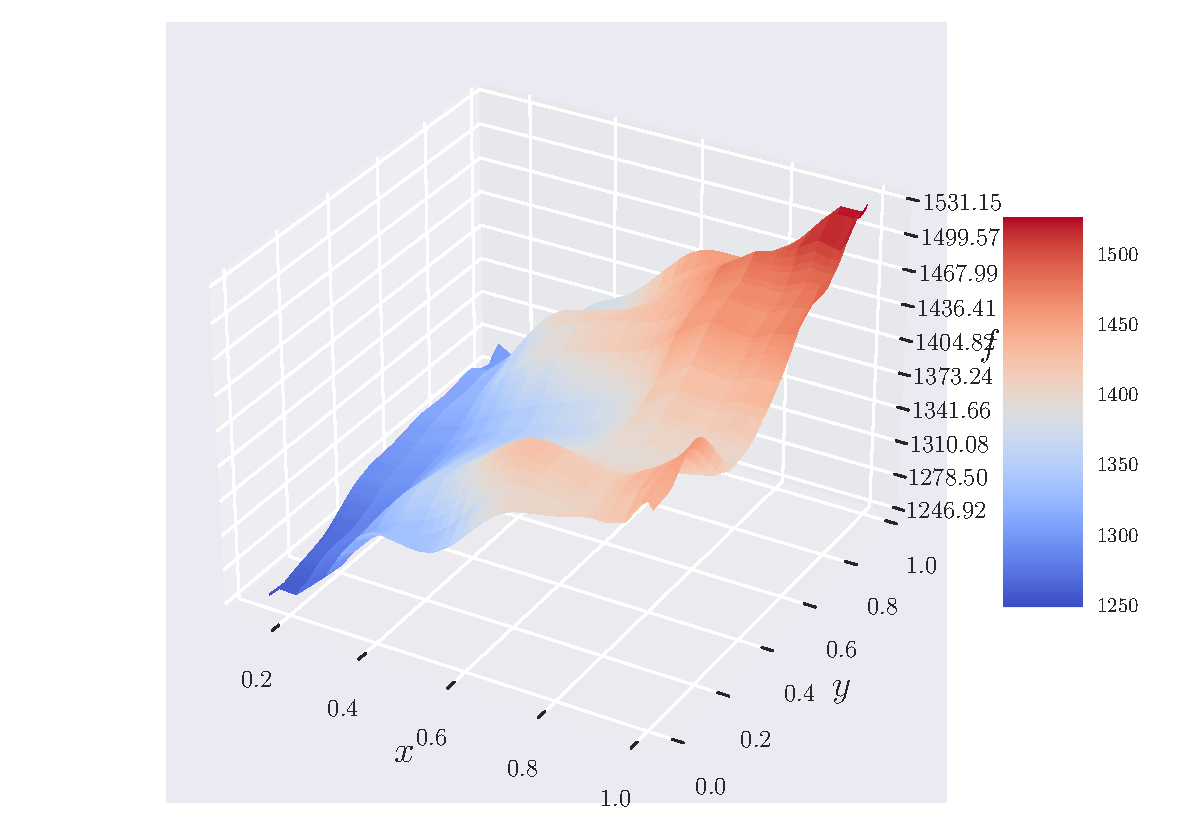
\includegraphics[width=\linewidth]{SRTM_prediction_p20.pdf}
	\endminipage\hfill
  \minipage{0.49\textwidth}
	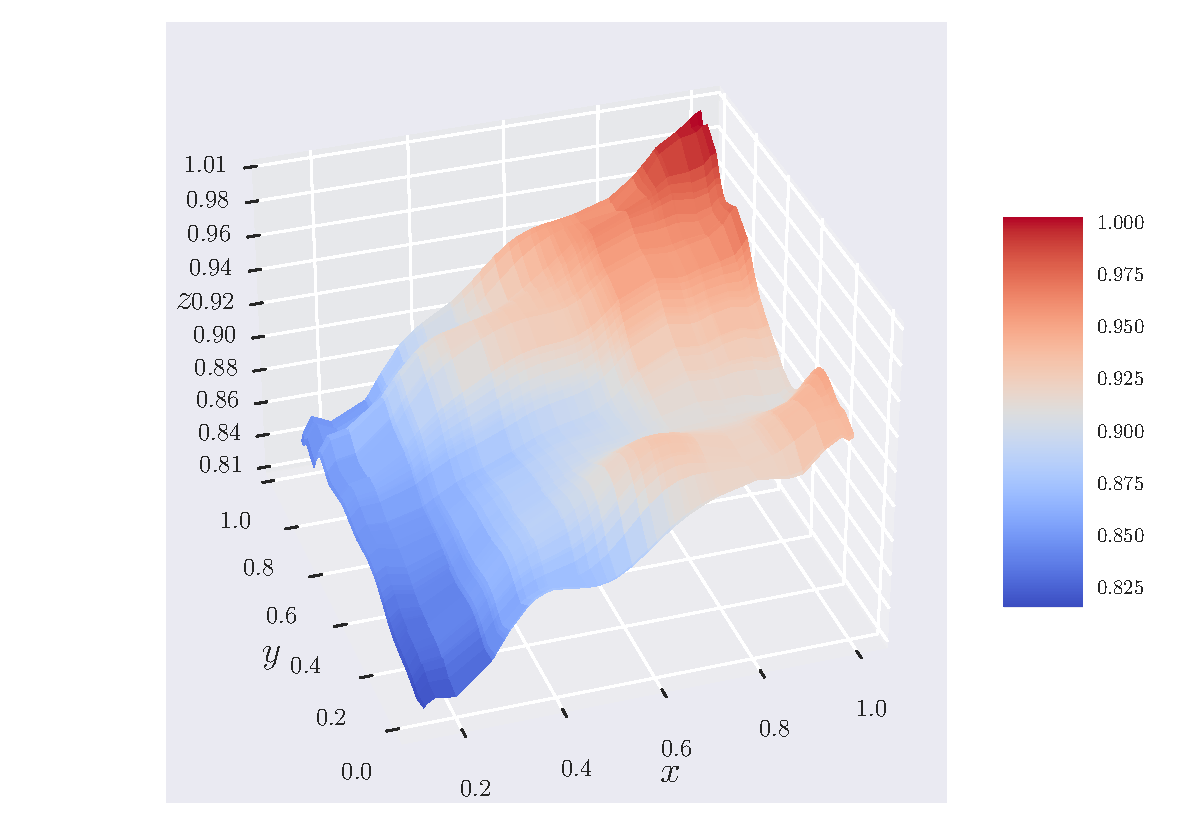
\includegraphics[width=\linewidth]{SRTM_prediction_p30.pdf}
	\endminipage\hfill
	\minipage{0.49\textwidth}
	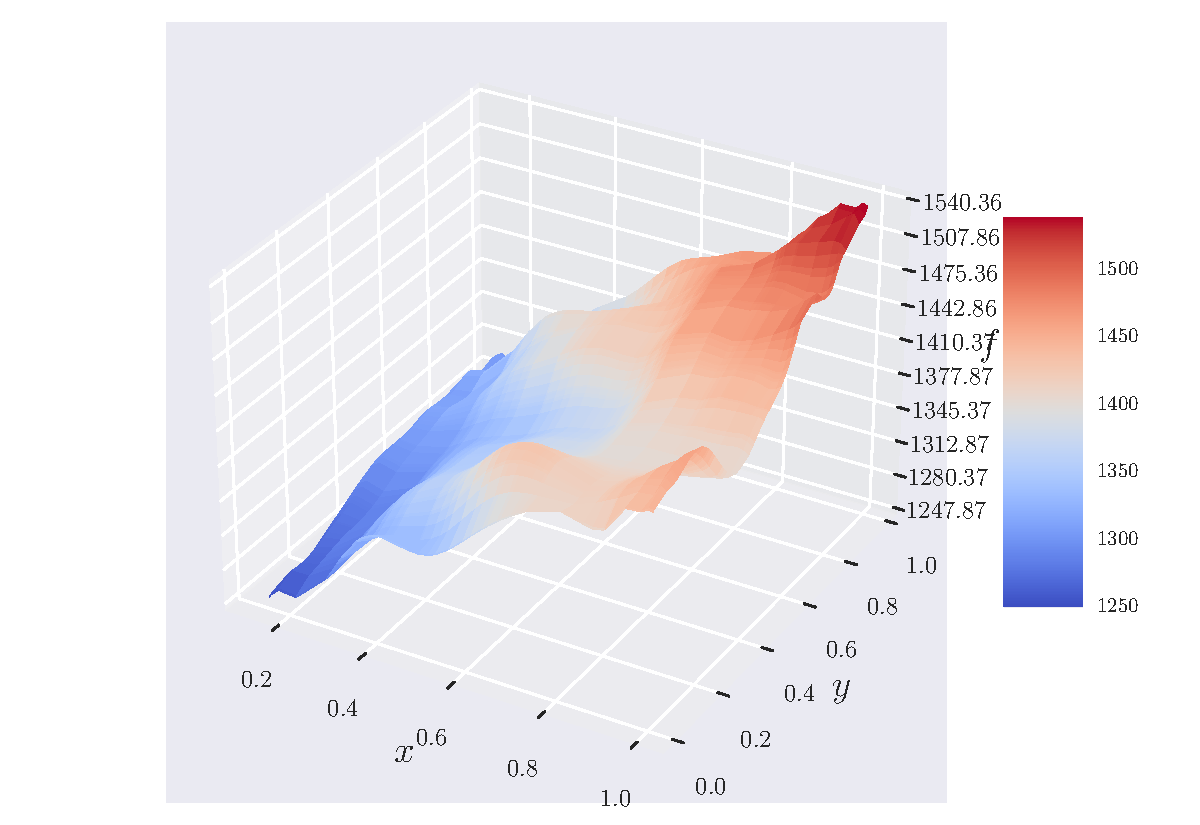
\includegraphics[width=\linewidth]{SRTM_prediction_p50.pdf}
	\endminipage
	\caption{Data til venstre. Fit til høyre}
  \label{fig:terrain_fit}
\end{figure}

In figure \ref{fig:terrain_fit} we see that $P=10$ gives a decent fit, as it encaptures the essential structure of the terrain. It does, however, miss out on essentially all of the rough details of the landscape. We also notice that important structures are missing, which can be seen from the missing elevation around $x=1$ and $y=0.8$, which is present in the other three fits. Using $P=20$ we are able to reproduce more nuanced structures, while most of the rough edges are still left out. Increasing up to $P=30$ does not change the fit much, other than a few more details at certain points. Finally, we study the resulting fit with $P=50$. Although it provides some more rough futures of the terrain, it illustrates some difficulties of the fitting. The shape of the mointain top at $x=1$ and $y=1$ is no longer consisitent with the original terrain data, and we git a tiny vally around $x=1$ and $y=0.8$, which is not an actual feature of the terrain data. Still, there are details missing along the $x$-axis at $y=1$, and the structure of the two peaks at $y=0$ is still not being represented accurately. We emphasize that the misrepresentations obtained with $P=50$ might be a consequence of the splitting of train and test data, as well as that prticalur ploynomial degree. However, we are still not able to accurately predict important structures of the terrain.

We also include a plot of the mean squared error with bootstrap resampling for each factor $5$ polynomial degree from $p=5$ up to $P=50$, shown in figure \ref{fig:terrain_MSE_bootstrap_p50}.

\begin{figure}[H]
  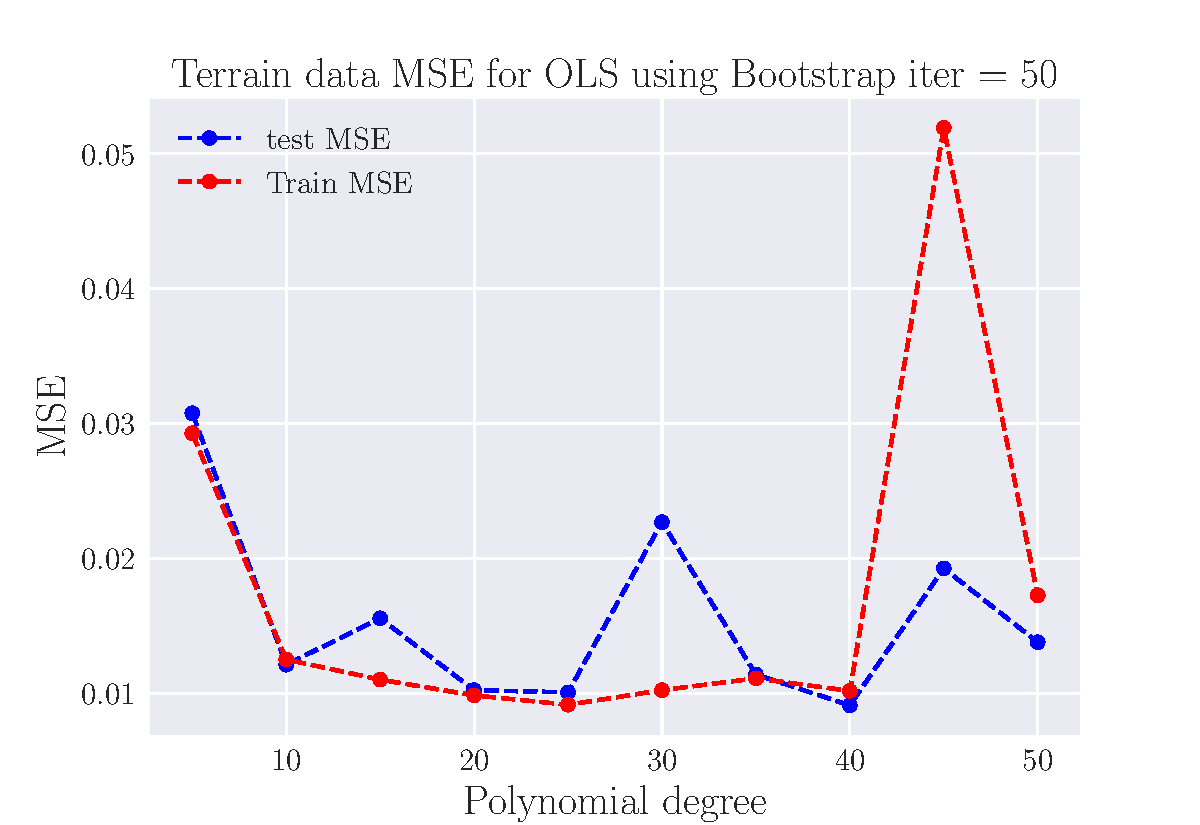
\includegraphics[width=\linewidth]{SRTM_MSE_OLS_n50_pol50_Bootstrap_re50.pdf}
  \caption{MSE}
  \label{fig:terrain_MSE_bootstrap_p50}
\end{figure}

This illustrates the difficulties of fitting this terrain data, as subtle structures will still be missing in our fitted model, despite using polynomial degrees where overfitting is taking place. Despite large fluctuations in the MSE for higher order polynomials, it's worth mentioning that the MSE values themselves are not particularly large, which is expected since we don't include noise in our data. !SJEKK!

Now, we move on the studying the MSE with the cross validation resampling method. To see the detailed behaviour of the MSE with cross-validation we restrict our analysis to $P=10$ as the maximum polynomial degree, since higher degrees caused the MSE to explode. The result of the cross-validation resampling is shown for $5$ and $10$ k-folds in figure \ref{fig:terrain_OLS_MSE_CV}.
\begin{figure}[H]
	\minipage{0.49\textwidth}
	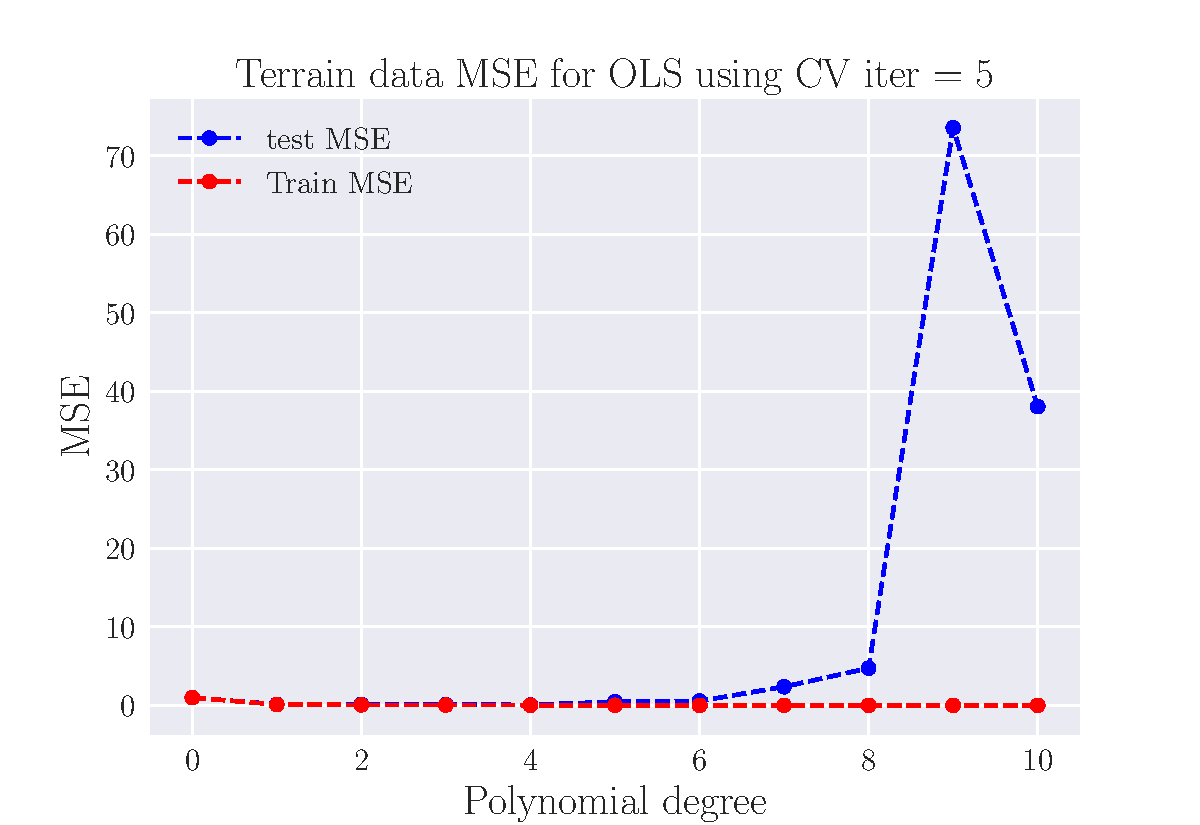
\includegraphics[width=\linewidth]{SRTM_MSE_OLS_n50_pol10_CV_re5.pdf}
	\endminipage\hfill
	\minipage{0.49\textwidth}
	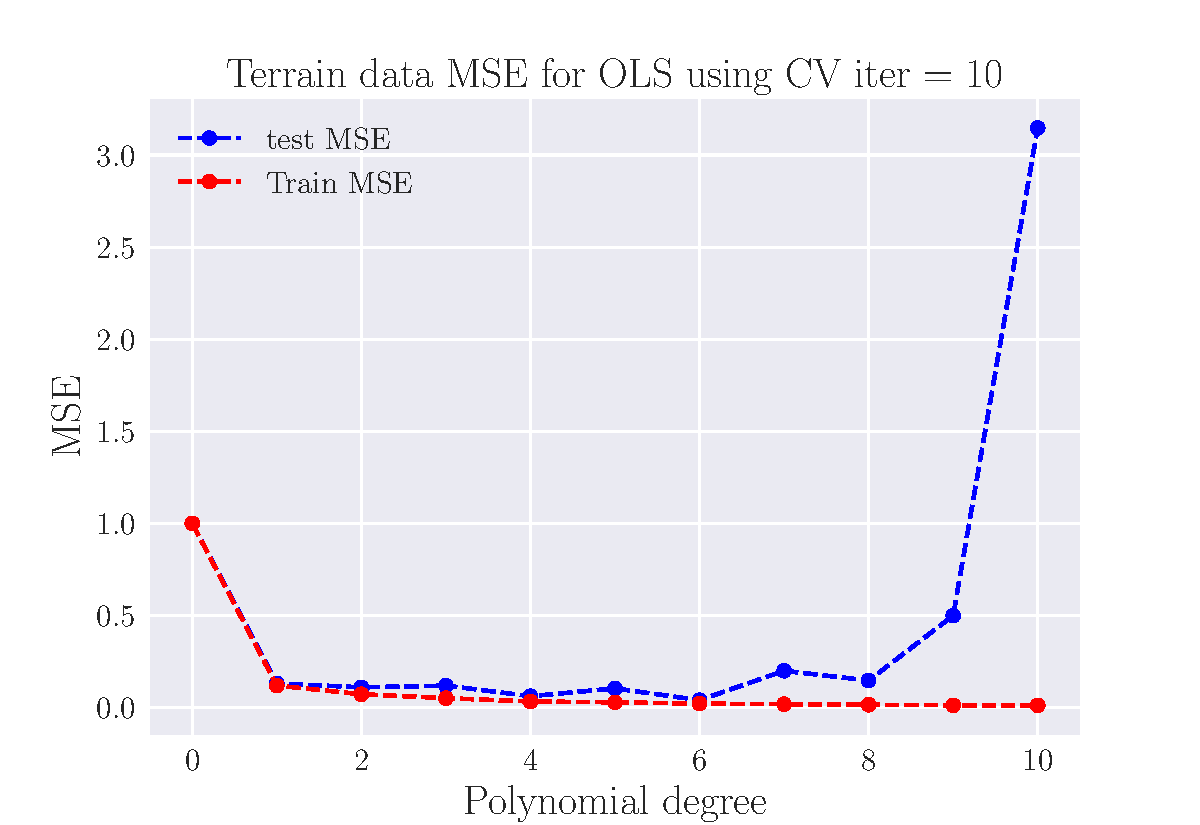
\includegraphics[width=\linewidth]{SRTM_MSE_OLS_n50_pol10_CV_re10.pdf}
	\endminipage
	\caption{k-fold 5 til venstre. k-fold 10 til høyre}
  \label{fig:terrain_OLS_MSE_CV}
\end{figure}
With $5$ k-folds, we see that the test MSE becomes incredibly large when $P>8$. Doubling the number of k-folds, the MSE drops significantly, but there is still a clear increase for $P>8$.
!Discussion/interpretation!

Using the bootstrap method for resampling, we perform a Bias-variance trade-off. Using $P=25$ as the largest polynomial, we are unable to see the relative behaviour of the quantities we plot for $50$ data points, so we use a logarithmic scale on the y-axis. The result is shown on the left panel in figure \ref{fig:terrain_OLS_BVT}. Once again, we include a result obtained with fewer data points to see any noticeable effect. The bias-variance trade-off result for $15$ data points is shown on the right panel of figure \ref{fig:terrain_OLS_BVT}, up to $P=10$. This clearly shows an increase in the test MSE and test variance as $P$ increases, while the bias declines.
\begin{figure}[H]
	\minipage{0.49\textwidth}
	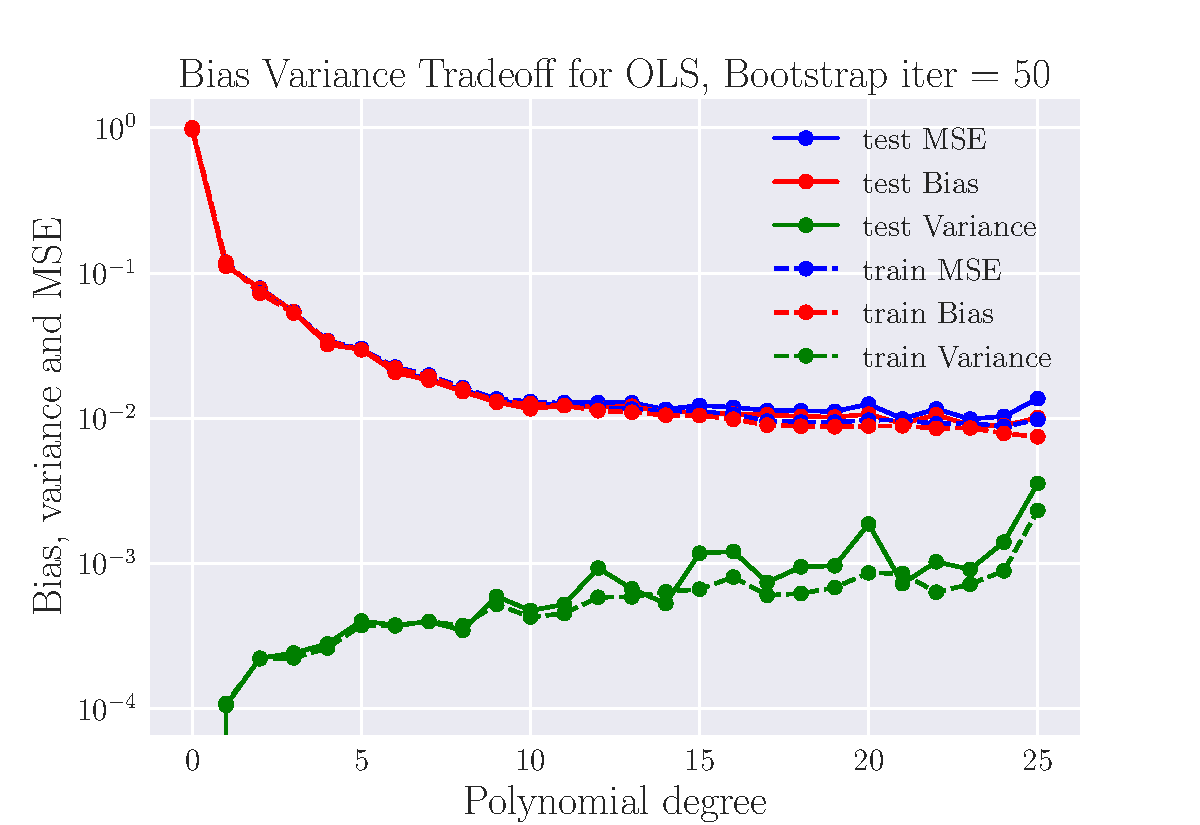
\includegraphics[width=\linewidth]{SRTM_BVT_OLS_n50_log.pdf}
	\endminipage\hfill
	\minipage{0.49\textwidth}
	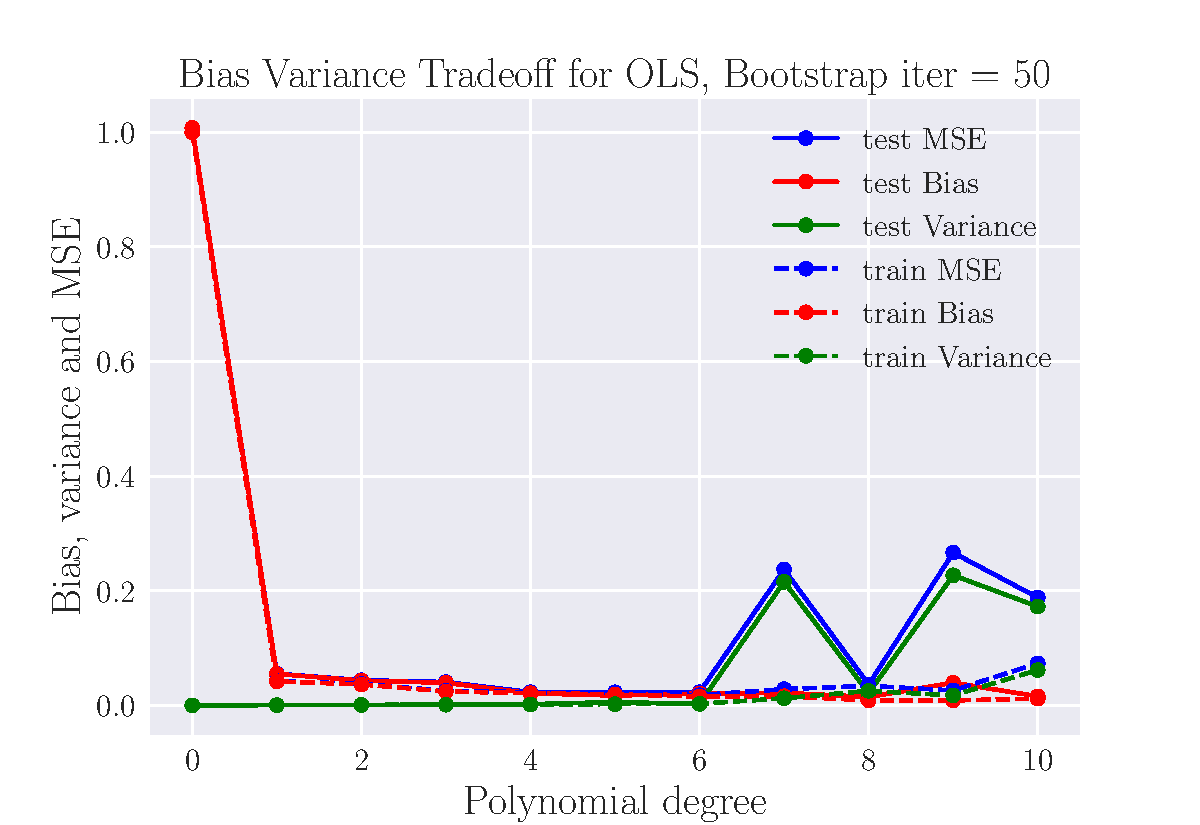
\includegraphics[width=\linewidth]{SRTM_BVT_OLS_n15.pdf}
	\endminipage
	\caption{n50 log til venstre. n15 til høyre}
  \label{fig:terrain_OLS_BVT}
\end{figure}


\appendix


\section{Bias-variance Decomposition}\label{Apx:BVT}

We assume that our true data is generated from a noisy model with nromally distributed noise $\epsilon$ with a mean of zero and standard deviation $\sigma^2$, i.e.
\begin{align*}
  \mathbf{y} &= f(\mathbf{x}) + \bm{\epsilon}
\end{align*}

We have approximated this function with our design matrix $\mathbf{X}$ and our parameters $\bm{\beta}$ such that our model becomes $\mathbf{\tilde{y}}=\mathbf{X}\bm{\beta}$, where the values of $\bm{\beta}$ were obtained by optimizing the mean squared error via the cost function, given by

\begin{align*}
  C(\mathbf{X}, \bm{\beta}) &= \frac{1}{n} \sum_{i=0}^{n-1} (y_i - \tilde{y}_i)^2 = \mathbb{E}\left[(\mathbf{y} - \mathbf{\tilde{y}})^2\right]
\end{align*}


where $\mathbb{E}$ is the expected value. % Note sample value

We want to show that the above expression can be written as

\begin{align*}
  \mathbb{E}\left[(\mathbf{y} - \mathbf{\tilde{y}})^2\right] &= \frac{1}{n} \sum_i (f_i - \expy)^2 + \frac{1}{n}\sum_i (\tilde{y}_i - \expy )^2 + \sigma^2
\end{align*}

We begin by inserting our model expression for $\mathbf{y}$ and adding and subtracting $\expy$ inside the expected value, before we square the expression.
\begin{align*}
  \mathbb{E}\bracket{(\mathbf{y} - \mathbf{\tilde{y}})^2} &= \mathbb{E}\bracket{(f(\mathbf{x}) + \bm{\epsilon} - \mathbf{\tilde{y}} - \expy + \expy)^2} = \mathbb{E}\bracket{\closed{(f(\mathbf{x}) - \expy) + \bm{\epsilon} + (\expy - \mathbf{\tilde{y}}) }^2 } \\
  &= \mathbb{E}\bracket{(f(\mathbf{x}) - \expy)^2 + \bm{\epsilon}^2 + (\expy - \mathbf{\tilde{y}})^2} \\
  &\quad+ \mathbb{E}\bracket{2\bm{\epsilon} (f(\mathbf{x}) - \expy) + 2\bm{\epsilon}(\expy - \mathbf{\tilde{y}}) + 2 (f(\mathbf{x}) - \expy)(\expy - \mathbf{\tilde{y}})}
\end{align*}

where the cross terms have been written on a separate line since the expected value is linear. Next we will focus on the cross-terms. Since $\bm{\epsilon}$ is normally distributed, it's expected value is simply the mean, which is zero in our case. The two cross terms involving $\bm{\epsilon}$ is therefore zero, so we only need to consider
\begin{align*}
  \mathbb{E}\bracket{(f(\mathbf{x}) - \expy)(\expy - \mathbf{\tilde{y}})} &= \mathbb{E}\bracket{f(\mathbf{x})\expy} - \mathbb{E}\bracket{f(\mathbf{x})\mathbf{\tilde{y}}} - \mathbb{E}\bracket{\expy\expy} + \mathbb{E}\bracket{\mathbf{\tilde{y}}\expy}
\end{align*}
Since the expected value of an expected value is just the expected value itself the last two terms in the above equation both become $\expy^2$, canceling each other out. Using that $f(\mathbf{x})$ is a deterministic function, we have $\mathbb{E}[f(\mathbf{x})]=f(\mathbf{x})$. Expressing $f(\mathbf{x})$ in terms of its expected value, we can write the first two terms in the above equation as
\begin{align*}
  \mathbb{E}\bracket{f(\mathbf{x})\expy} - \mathbb{E}\bracket{f(\mathbf{x})\mathbf{\tilde{y}}} &= \mathbb{E}\bracket{\mathbb{E}\bracket{f(\mathbf{x})}\expy} - \mathbb{E}\bracket{\mathbb{E}\bracket{f(\mathbf{x})}\mathbf{\tilde{y}}} \\
  &= \mathbb{E}\bracket{f(\mathbf{x})}\expy - \mathbb{E}\bracket{f(\mathbf{x})}\expy = 0
\end{align*}

Hence, all the cross terms in the expected value cancel out, and we're left with
\begin{align*}
  \mathbb{E}\left[(\mathbf{y} - \mathbf{\tilde{y}})^2\right] &= \mathbb{E}\bracket{\closed{f(\mathbf{x})-\expy}^2} + \mathbb{E}\bracket{\closed{\expy - \mathbf{\tilde{y}}}^2} + \mathbb{E}\bracket{\bm{\epsilon}^2}
\end{align*}

Using that $\mathbb{E}[\epsilon^2]=\sigma^2$ and writing the expected values as sums with the notation $f(\mathbf{x}_i)=f_i$, we get the desired expression. Since we have chosen $\mathbf{z}$ as our data variable we replace all the $y$ variables with $z$, yielding
\begin{align}
  \mathbb{E}\left[(\mathbf{z} - \mathbf{\tilde{z}})^2\right] &= \frac{1}{n} \sum_i (f_i - \expz)^2 + \frac{1}{n}\sum_i (\tilde{z}_i - \expz )^2 + \sigma^2
\end{align}
which is what we wanted to show.

\section{Testing our implementation}\label{Apx:test}
In order to make sure our algorithms are running correctly, it is necessary to perform tests. We did this by comparing our results to those produced by scikit-learn. First of all we generated some simpler data for testing:
\begin{equation}
	\label{eq:test_data}
	y = \exp{-x^2} + 1.5\cdot\exp{-(x-2)^2} + \epsilon.
\end{equation}

Here $\epsilon$ denotes normally distributed noise with zero mean and variance $\sigma^2 = 0.1$. We look at when $x$ runs from $x_\text{min} = 0$ to $x_\text{max} = 1$ in $N = 50$ randomly distributed steps. This generates the testing data visualized in figure \ref{fig:TestingData}.

\begin{figure}[H]
	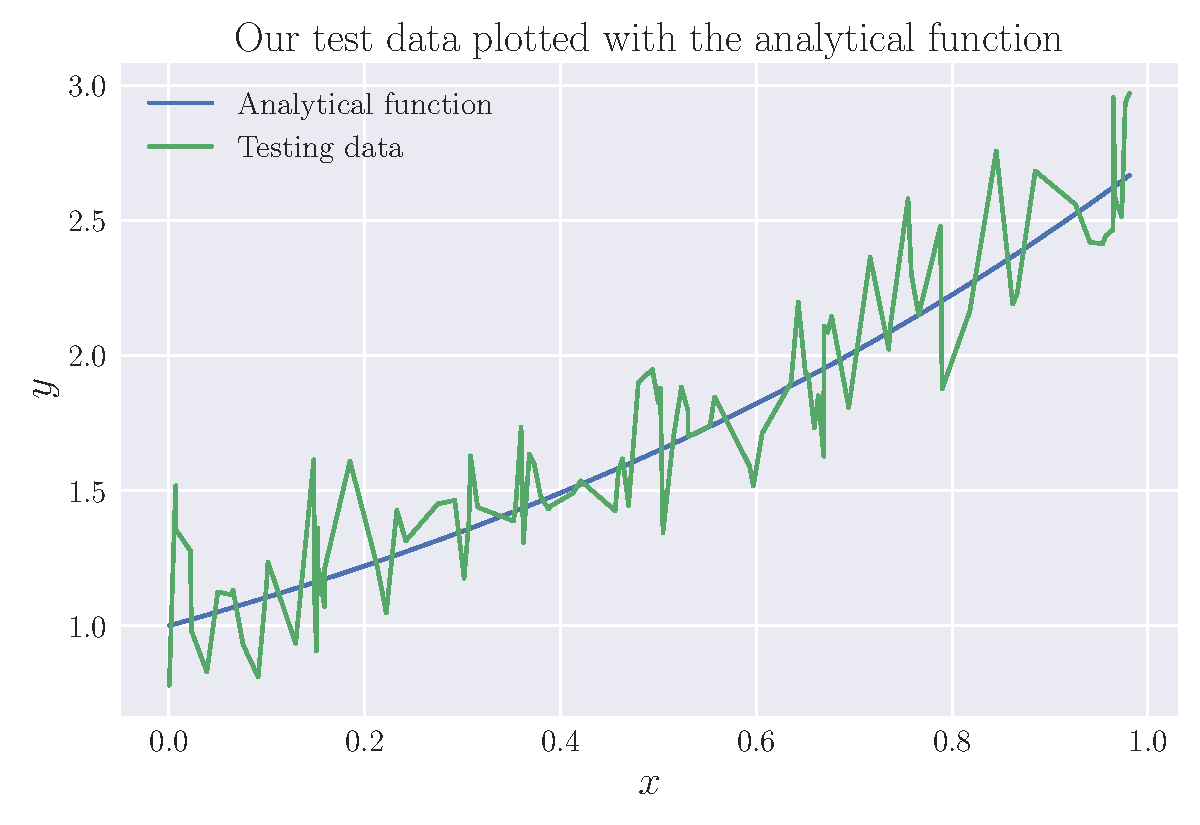
\includegraphics[width=\linewidth]{Testing_data.pdf}
	\caption{Here you we have plotted the testing data along with the analytical function. The solid blue line denotes the analytical function.}
	\label{fig:TestingData}
\end{figure}

We test the implementation of OLS and Ridge regression. For Lasso we already used the scikit-learn implementation, so there is no reason to compare it with itself.
\begin{figure}[H]
	\minipage{0.49\textwidth}
	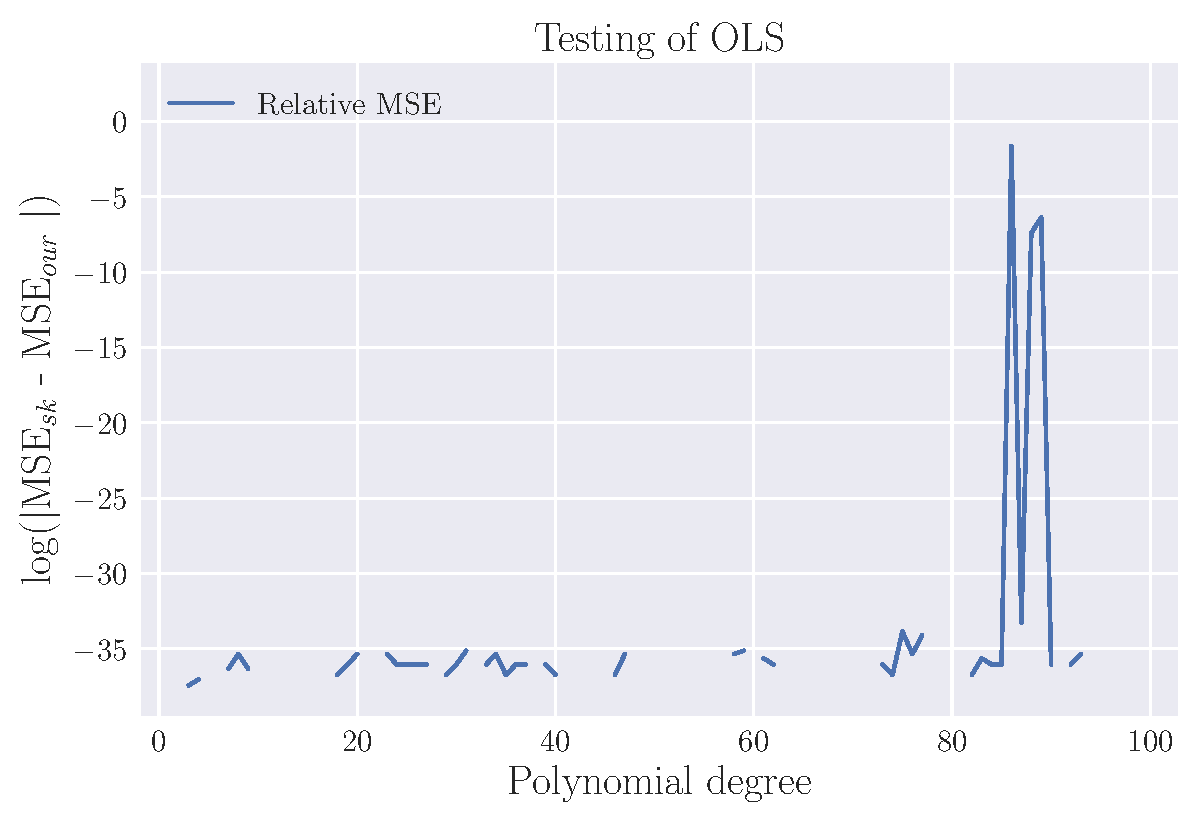
\includegraphics[width=\linewidth]{Testing_OLS.pdf}
	\endminipage\hfill
	\minipage{0.49\textwidth}
	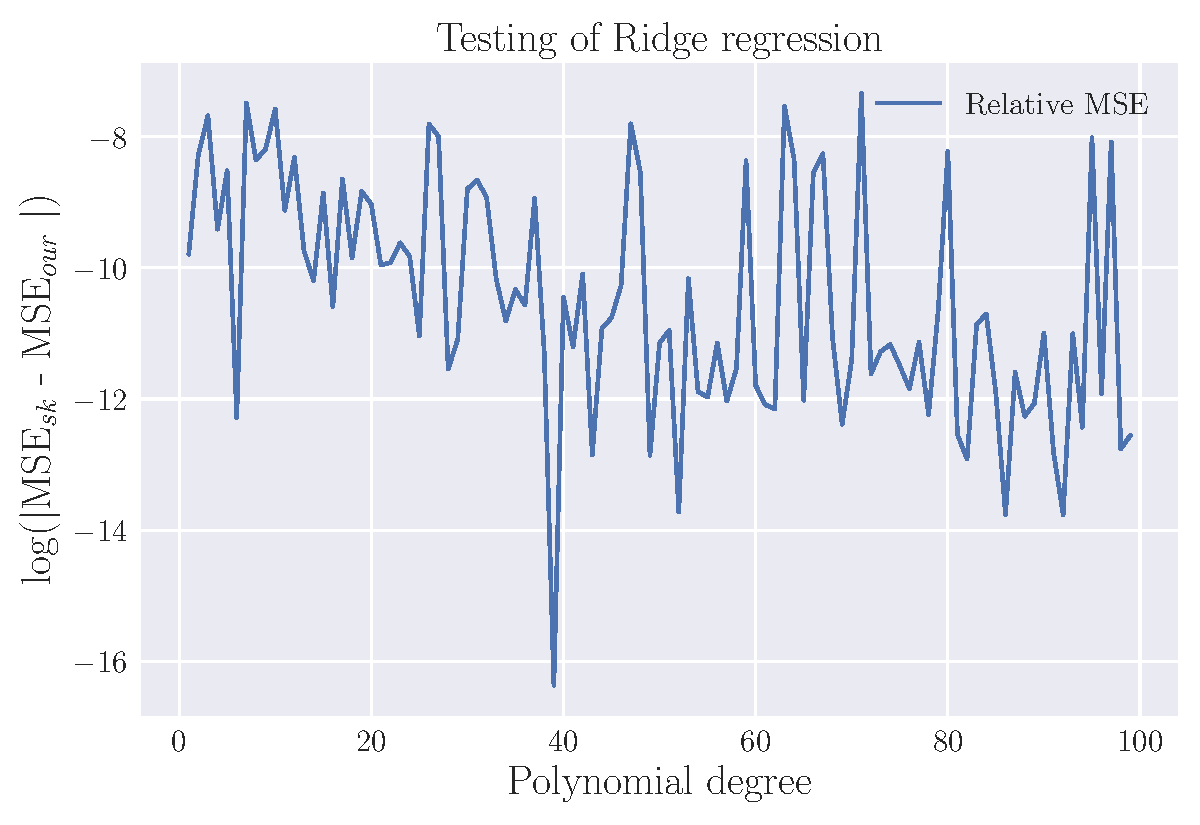
\includegraphics[width=\linewidth]{Testing_Ridge.pdf}
	\endminipage
	\caption{In this figure we have plotted the test and train MSE for both OLS (left plot) and Ridge regression (right plot). Along the $x$-axis we have polynomial degree, and MSE along the $y$-axis. The blue and red dashed line is the sklearn MSE respectively. We plotted our test and train MSE as red and blue dots respectively.}
	\label{fig:test_OLS_Ridge}
\end{figure}
Looking at figure \ref{fig:test_OLS_Ridge}, our OLS implementation returns indistinguishable MSE's compared to sklearn. For ridge however we see some small deviations at polynomial degrees $p=7$ and $p = 13$. The strong correspondence makes us confident that our implementations are correct, however, we one should be wary that our results deviate at some polynomial degrees. This is probably due to optimizations that the professional library sklearn has done.


\section{Testing Bias Variance Tradeoff}\label{Apx:testing_BVT}
To ensure a correct implementation of the Bias Variance tradeoff for the Bootstrap method, we want to compare our implemented results with results obtained by scikitlearn. This will also provide us insight of how these results behave. We consider the same data as when we tested our regression methods in Appendix \ref{Apx:test} (equation \eqref{eq:test_data}). However with a slightly different domain, namely $x\in[-3,3]$.

When we compare our own results with the ones obtained from scikitlearn, the result depends a lot on the particular setup we consider. We use $4/5$ of our data as the training data, $100$ bootstrap iterations and polynomial degrees from $P=0$ up to $P=15$ and scale this data by subracting the mean before dividing by the standard deviation. The differences we see between when we compare are very sensitive to the configuration. To illustrate this, we first perform the bias variance tradeoff with $N=170$ data points and then with $N=169$ data points. The resulting plots for the two configuration are shown in figure \ref{fig:compare_BV_scikit}, on the left and right panel, respectively.

\begin{figure}[H]
  \minipage{0.49\textwidth}
  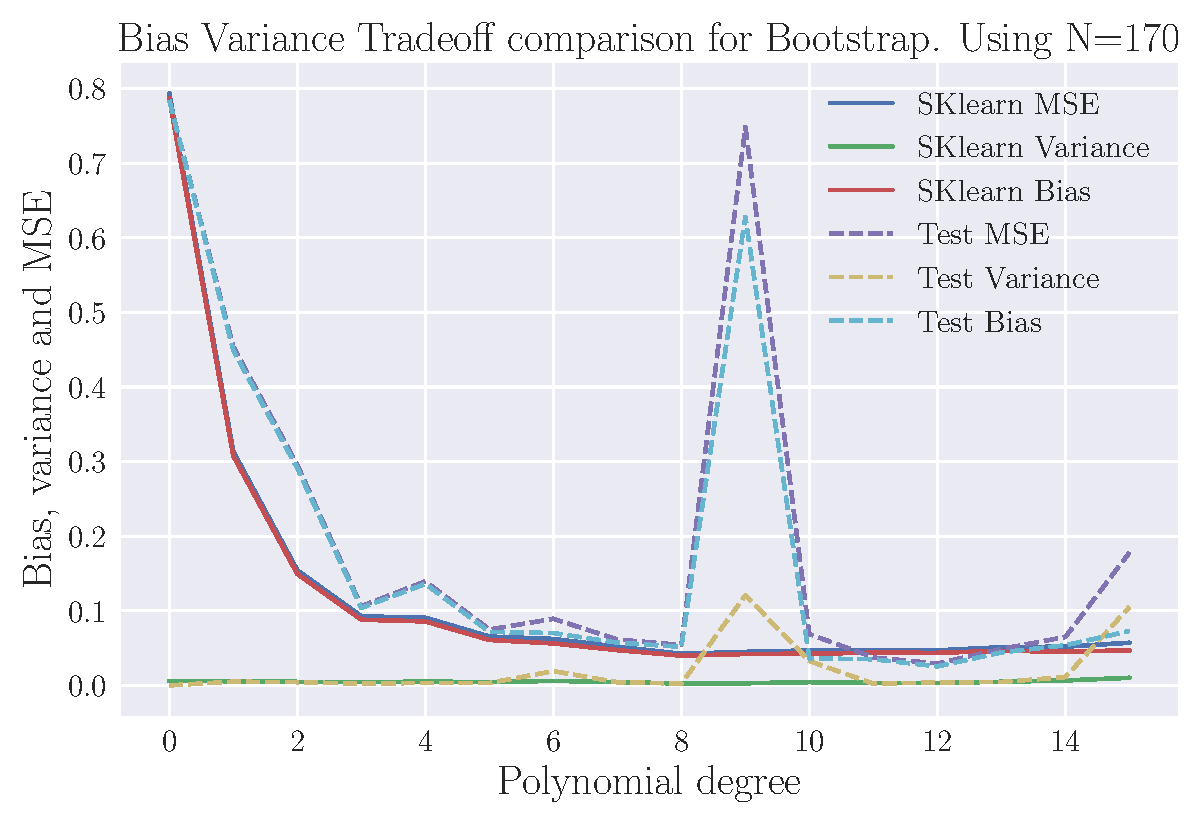
\includegraphics[width=\linewidth]{Testing_OLS_BV_compare_n170.pdf}
  \endminipage\hfill
  \minipage{0.49\textwidth}
  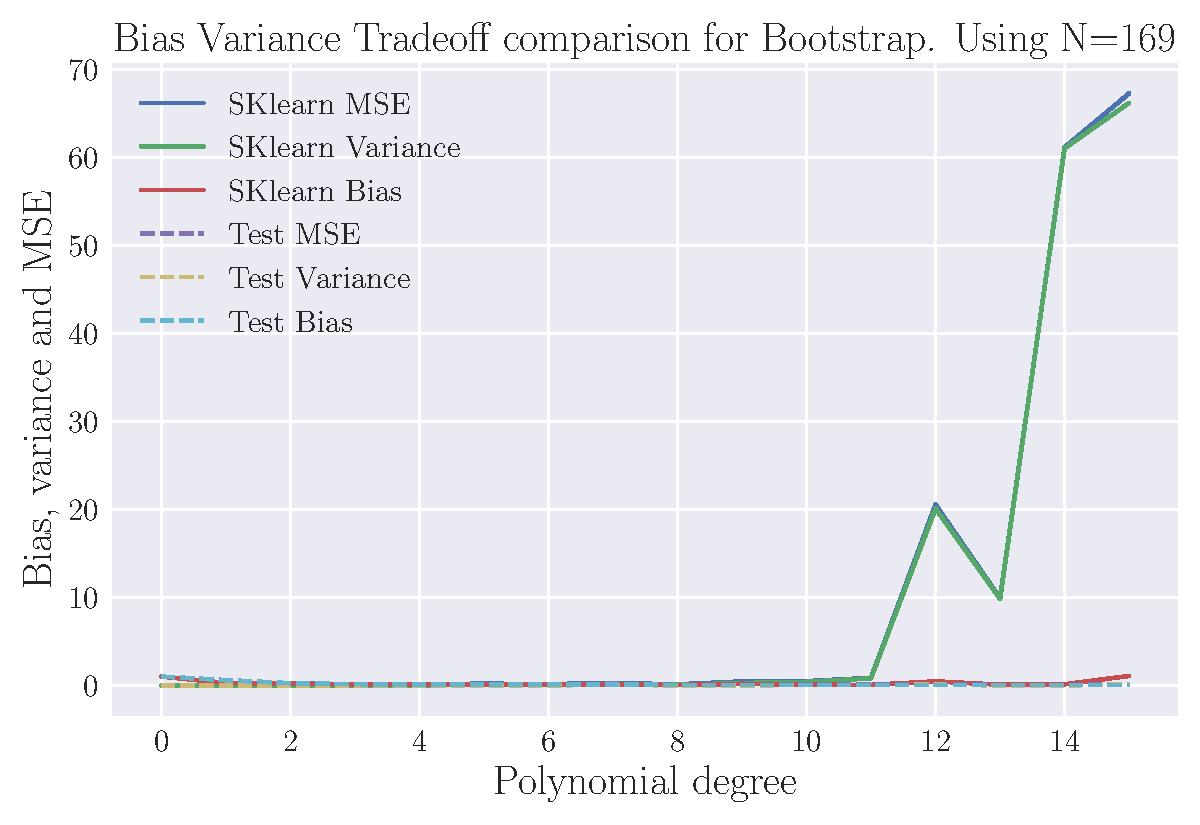
\includegraphics[width=\linewidth]{Testing_OLS_BV_compare_n169.pdf}
  \endminipage
  \caption{BV compare}
  \label{fig:compare_BV_scikit}
\end{figure}

For $N=170$ data points, our model yields a low variance and a high bias and MSE at first, similar to scikit-learn, just as expected. For a polynomial degree of $P=9$, we get an abrupt increase ouf our three metrics while scikit-learn remains stable. For $P=15$ we see that our variance and MSE starts to increase, while the bias remains low, just as desired. This feature is less present for the scikit-learn. If we compare with $N=169$, as shown on the right panel in figure \ref{fig:compare_BV_scikit}, we see that the variance and MSE of the scikit-learn model exceeds a value of $60$ for $P>14$, which is not present in our model. This shows that the bias variance trade-off is generally sensitive to our particular configuration, so when performing a bias-variance trade-off analysis on the Franke function our result may be correct, despite odd behaiour for certain polynomial degrees.

\begin{thebibliography}{}
\bibitem[]{ref} Ref.

\end{thebibliography}


\end{document}
